\documentclass[review,authoryear]{elsarticle}
%\documentclass[12pt]{article}
\usepackage{lineno,hyperref}
\usepackage{graphicx}
\usepackage[margin=2cm]{geometry}

\pdfstringdefDisableCommands{%
%  \def${}%
  \def\alpha{alpha}%
  \def\({}%
  \def\){}%
  \def\texttt#1{<#1>}%
}
\usepackage{amsmath}
\usepackage{amssymb}
\usepackage{amsthm}
\usepackage{xcolor}
\newtheorem{theorem}{Theorem}[section]
\newtheorem{lemma}[theorem]{Lemma}
\newcommand{\origB}{{b}}
\newcommand{\origW}{{w}}
\newcommand{\origAlpha}{{\alpha}}
\newcommand{\origK}{{K}}
\newcommand{\origGamma}{{\gamma}}
\newcommand{\origA}{{a}}
\newcommand{\origC}{{c}}
\newcommand{\origD}{{d}}
\newcommand{\origG}{{g}}
\newcommand{\origL}{{L}}
\newcommand{\origP}[1]{{p}(#1)}
\newcommand{\origTheta}{{\theta}}
\newcommand{\origT}{{t}}
\newcommand{\origMu}{{\mu}}

\newcommand{\scaledB}{\hat{b}}
\newcommand{\scaledW}{\hat{w}}
\newcommand{\scaledAlpha}{\hat{\alpha}}
\newcommand{\scaledK}{\hat{K}}
\newcommand{\scaledGamma}{\hat{\gamma}}
\newcommand{\scaledA}{\hat{a}}
\newcommand{\scaledC}{\hat{c}}
\newcommand{\scaledD}{\hat{d}}
\newcommand{\scaledG}{\hat{g}}
\newcommand{\scaledL}{\hat{L}}
\newcommand{\scaledP}[1]{\hat{p}(#1)}
\newcommand{\scaledTheta}{\hat{\theta}}
\newcommand{\scaledT}{\hat{t}}
\newcommand{\scaledMu}{\hat{\mu}}
\newcommand{\scaledM}{\hat{m}}


\modulolinenumbers[5]
% https://www.overleaf.com/project/5eb9da10e929ab0001816b1e
\journal{Ecological Modeling}

%%%%%%%%%%%%%%%%%%%%%%%
%% Elsevier bibliography styles
%%%%%%%%%%%%%%%%%%%%%%%
%% To change the style, put a % in front of the second line of the current style and
%% remove the % from the second line of the style you would like to use.
%%%%%%%%%%%%%%%%%%%%%%%

%% Numbered
%\bibliographystyle{model1-num-names}

%% Numbered without titles
%\bibliographystyle{model1a-num-names}

%% Harvard
%\bibliographystyle{model2-names.bst}\biboptions{authoryear}

%% Vancouver numbered
%\usepackage{numcompress}\bibliographystyle{model3-num-names}

%% Vancouver name/year
%\usepackage{numcompress}\bibliographystyle{model4-names}\biboptions{authoryear}

%% APA style
%\bibliographystyle{model5-names}\biboptions{authoryear}
%%https://www.overleaf.com/project/5eb9da10e929ab0001816b1e
%% AMA style
%\usepackage{numcompress}\bibliographystyle{model6-num-names}

%% `Elsevier LaTeX' style
%\bibliographystyle{elsarticle-num}
%%%%%%%%%%%%%%%%%%%%%%%


%% Available colors:  black, blue, brown, cyan, darkgray, gray, green, lightgray, %lime, magenta, olive, orange, pink, purple, red, teal, violet, white, yellow.
\begin{document}

\begin{frontmatter}

\title{A Continuous Model Of Behavioural Phenotype: An Example Of
  Interaction Between The Butterfly \textit{Pieris brasicae} And
  \textit{Trichogramma} Wasps}
%\tnotetext[mytitlenote]{Fully documented templates are available in the elsarticle package on \href{http://www.ctan.org/tex-archive/macros/latex/contrib/elsarticle}{CTAN}.}

%% Group authors per affiliation:
\author[math]{Kelly Black\fnref{myfootnote}}\author[math]{Malcolm R Adams}\author[math]{Aladeen Al Basheer}\author[math,engineering]{Caner Kazanci}\author[odum]{Bernard Patten}\author[odum]{Stuart Whipple}\author[math]{Sofya Zaytseva}

\fntext[myfootnote]{Corresponding author, kjblack@gmail.com}
\address[math]{Department of Mathematics, University of Georgia, Athens, GA 30602, USA}
\address[engineering]{College of Engineering, University of Georgia, Athens, GA 30602, USA}
\address[odum]{Odum School of Ecology and College of Engineering, University of Georgia, Athens, GA 30602, USA}



\begin{abstract}
TO DO: include an abstract
Discuss diffusion!
\end{abstract}

\begin{keyword}
behavioral phenotype, genetic variation, population dynamics, group phenotypic composition
\end{keyword}

\end{frontmatter}

\linenumbers


\section{Introduction}

A wide variation in animal behaviours as well as the variation in the corresponding genetic basis for animal personalities play a large role in species interactions \citep{doi:10.1111/j.1461-0248.2010.01536.x,doi:10.1086/687235,mierzejewski_horn_luong_2019,SANTICCHIA20191,doi:10.1098/rspb.2014.1016,FARINE2015609,sibbald2009individual,kurvers2011effect,modlmeier2012diverse,doi:10.1037/0735-7036.107.3.250}.   Recognition for this important phenomenon continues to growa, and several techniques, including compartment models, stochastic
models, agent based models, and combinations of these
approaches, have been developed to explore this important aspect of species interactions  \citep{Keeling65,doi:10.1086/687235,doi:10.1098/rspb.2001.1599,SuperspreadingLloyd}.  One difficulty, though, with these approaches is the challenge of developing appropriate analytic models that feature a wide range of behavioural manifestations with fine resolution. Refining the resolution by increasing the number of levels representing the differences in animal behavior in a compartment model or an agent based model can make it more difficult to interpret and analyze the resulting system of equations. 

We propose a novel approach that assumes a continuous distribution
associated with a single behavioural aspect of an animal's behaviour. The temporal dynamics of the distribution is modeled as a diffusion process. In contrast to the widespread use of diffusion to model animal movement in space, the presented model uses diffusion to model the evolutionary processes that maintain the variation in animal behavior. In
this initial exploration of this approach, we choose to model a relatively
straight-forward interaction in order to explore its viability. Our model is based on
the interactions between parasitic wasps of the genus
\textit{Trichogramma}, and the butterfly \textit{Pieris
  brasicae} \citep{10.1093/beheco/arq007}.  The propensity of
\textit{Pieris brasicae} to employ a chemical associated with mating
behaviour is modeled as a continuous distribution.

While the original system of interactions involves multiple species, we consider a simplified system consisting of two species, butterflies and wasps. The interaction between the two species depends on a pheromone that can be used by the males of the butterfly population. The pheromone associated with mating is meant to give the butterflies a benefit in survival, but paradoxically it is also an attractant for the wasp, which parasitizes the eggs. The two opposing pressures on the butterflies' use of the chemical provide a context to examine how the expression of this behavior can evolve in time. Modeling the use of pheromone as a continuous diffusion process provides the opportunity to investigate the interaction between the distribution of this behavior and population dynamics at a fine resolution.

Our discussion of these interactions is organized as follows. In section 2 we  provide a more detailed overview of behavioural phenotypes
including some previous efforts to model the phenomena. Next, in section 3, a model composed of a coupled partial differential equation (PDE) and ordinary differential equation (ODE) is derived. 
In section 4, a related, simplified ODE model is introduced to help provide insight into the
long term behaviour of the solution to the model. Following the introduction of the ODE model, an equilibrium analysis of the new system is explored. Finally, some results from our numerical explorations are provided including notes of the ecological implications. Separate appendices are included with a more detailed analysis of the model as well as details on the numerical approximation of the full model.

\section{Behavioral Phenotype}
\label{section:behaviouralPhenotype}

In this section we begin with a discussion of the basic idea of behavioural phenotype and its importance in population dynamics. A number of examples from the literature of observed behavioural variation are discussed and several modeling efforts from the literature are briefly described.


A number of authors have noted the importance of variation
in a species' habits or
genetics \citep{doi:10.1111/j.1461-0248.2010.01536.x,doi:10.1086/687235,mierzejewski_horn_luong_2019,SANTICCHIA20191,doi:10.1098/rspb.2014.1016}. This variation is sometimes referred to as group phenotypic composition \citep{FARINE2015609}, and it is observed in many species of animals such as sheep, barnacle geese, ants, spiders, fish and wild birds among others \citep{sibbald2009individual,kurvers2011effect,modlmeier2012diverse,doi:10.1086/687235,doi:10.1098/rspb.2014.1016,doi:10.1037/0735-7036.107.3.250}.
A broad discussion by  \citep{doi:10.1111/j.1461-0248.2010.01536.x} includes a description of variation in behavioural traits with multiple examples of the different ways it can impact a population. An example of variation in behaviours includes varying levels of boldness which can result in different levels of exposure to potential predation. Another example is the varying levels of social interaction within a colony of result in different rates of transmissions of disease or parasites between individuals. It is proposed that the diversity of
behaviours can profoundly impact the broader dynamics of the local populations as well as external populations that interact with them.


% https://www.semanticscholar.org/paper/Fish-behavioral-types-and-their-ecological-Mittelbach-Ballew/a381cb0b64a8107c694454e940fd7972263a8b77
% https://www.semanticscholar.org/paper/Are-most-samples-of-animals-systematically-biased-Biro/72eaa11f60d3b211f34ab04ff95211307978223b

Another example is provided by \cite{doi:10.1098/rspb.2014.1016} in a study of the effect of individual-level personality traits on the collective movement and feeding behavior of wild birds. In particular, they investigated the effects of patch-level behaviour variations of two different personality types - reactive individuals that displayed low-risk behavior and proactive individuals that displayed high-risk behavior. They found that patches of reactive individuals were more likely to choose a single foraging location to minimize the risk of predation, and patches of proactive individuals were more likely to disperse. The groups that contained a combination of the two types showed both group cohesiveness and patch exploration, indicating that behavioral variation can lead to better overall success, as was previously found in other animals such as ants and spiders \citep{ doi:10.1086/687235,modlmeier2011productivity,modlmeier2012diverse}.

A wide array of approaches to model the population responses to behaviour variation has been explored.  These include stochastic
models \citep{Keeling65}, agent based models \citep{doi:10.1086/687235},
hybrid models employing compartment models based on a stochastic
distribution \citep{doi:10.1098/rspb.2001.1599}, and statistical
models \citep{SuperspreadingLloyd}. A brief description of some of these
approaches is provided below.

An example of a stochastic model is provided by \cite{Keeling65}. They note that the dynamics of the incidence
of measles is influenced by how the incubation time varies across
individuals. 
They examine the impact of variation and the distribution associated with the variation in incubation times for the frequency of infectious outbreaks.
In response to this observation, they modify a standard
disease model by incorporating a time delay of the infected class using a convolution.  They note that the distribution associated with the variation plays an important role in determining the frequency of outbreaks.


Another adaptation for a similar problem was proposed by \cite{doi:10.1098/rspb.2001.1599}. In this case the rate at which
infected individuals leave the infected class is based on a stochastic
distribution. The phenomenon was modeled by making use of a large
number of compartments representing infected classes with different removal rates, where the entry into the different classes is
governed by the underlying probability distribution.

An example of a statistical approach that highlights the importance of
responses to individual variation is given by \cite{SuperspreadingLloyd}, where they investigate the influence of individual variation in infectiousness on disease emergence. In their work the transmission of
disease is examined using a branching process. The varying
transmission rates between individuals are treated as a given
probability distribution. They find that model predictions accounting for the individual variation differ sharply from average-based approaches for the estimation of transmission rates, which is often the case for models containing non-linear interactions such as the butterfly-wasp model presented in this paper, and predator-prey systems in general.

A mathematical model examining the interactions within a colony of
social spiders, \textit{Stegodyphus dumicola}, is provided by \cite{doi:10.1086/687235}. They  examine the impact of different boldness levels of
 key individuals on the success of the colony.  They note a small number of individuals within
a colony may exhibit different levels of aggression, and this small
number of individuals can have a disproportionate impact on the
broader success of the colony. This observation is a strong motivator for analyzing the interplay between the shape of the distribution of animal behavior and population dynamics, and how they affect each other. These observations provide additional motivation for our PDE model, which would offer unlimited resolution for both temporal dynamics and animal behavior for detailed analysis.

As a means to model this important aspect of a colony, \cite{doi:10.1086/687235} provide a computational model
consisting of an agent based model with a stochastically generated
population. Their approach is based on a small number of rules that
result in a distribution of behaviours. The temporal interactions
within the colony are approximated via discrete time steps and
stochastic decision making. The external interactions are approximated
using an ordinary differential equation model.
In the resulting statistical analyses, \cite{doi:10.1086/687235} found that different levels of boldness
within key individuals resulted in broad impacts across the colony. For example, one difference that was noted is that the variation in
boldness across indviduals impacted the prey capture rate for the whole colony. Another difference noted is that
the rules governing the distribution of aggression also impacted the spread of disease across the broader population.

The differences noted above represent a challenge with respect to measuring and detecting individual variation experimentally \citep{doi:10.1037/0735-7036.107.3.250}. In addition, 
many of the existing mathematical models that account for individual variation have been
developed in the context of the spread of an infectious disease. Only
a few approaches have been described for predator-prey systems, and
the majority of such models have been derived from statistical or
agent based approaches. The model presented here is a departure from
such approaches and offers a novel deterministic method.


\section{Modeling Genetic Variance As a Continuous Distribution}

Rather than a discrete or a continuous compartmental model or an agent based model, a
coupled partial differential equation model with a continuous, distributed parameter representing individual variation is proposed. First, an overview of the specific system, the interactions
between butterflies and parasitic wasps, is given. Next, the
model is derived, and the analysis of a simplified system of
ordinary differential equations (ODE) is examined as a way to gain some
preliminary insights into the coupled partial differential equation model. Finally, numerical results of the coupled partial differential equation (PDE) model are presented in parameter ranges informed by the ODE model.

\subsection{Butterflies v. Wasps}
\label{butterflyVWasps}

The model developed here focuses on the interaction between butterflies,
\textit{Pieris brasicae}, and \textit{Trichogramma} wasps that prey on
the butterflies' eggs. The interactions between these populations have
received a good deal of attention
\citep{PMC2797620,doi:10.1111/j.1439-0418.1986.tb00834.x,Figueroa2010AttractionOT,10.3389/fpls.2019.01768}. We
focus on the results of \cite{10.1093/beheco/arq007}. In their work, the authors state
that the pressure placed on the butterfly population due to the wasps'
interactions results in a change in the long term behaviour of the
butterfly population.

The source of this pressure is the nature of the mating practices of
\textit{Pieris brasicae}. In order to attract a mate, the female
butterflies tend to emit a pheromone designed to attract the males to
the females. After copulation, though, it is not in either the
female's nor the male's best interest to continue to attract other
butterflies. In response, the male butterflies have a propensity to
apply another pheromone, referred to as an anti-aphrodisiac, that will
reduce the effectiveness of the original pheromone emitted by the
female.
The downside to the use of the pheromone is that it exposes the eggs
to a greater risk of predation, as some species of \textit{Trichogramma}
wasps parasitize the eggs of the butterflies. Sometimes they
physically attach themselves to a butterfly and ride it until the
butterfly begins to attach their eggs in a preferable location. The
wasps are able to detect the presence of the anti-aphrodisiac which benefits the wasp, as a butterfly with the
anti-aphrodisiac is more likely to lay eggs. In response, the wasps
are more likely to ride on a butterfly if they detect the
anti-aphrodisiac. It is important to note that this method of predation on
a butterfly's eggs requires a non-trivial time commitment with respect
to handling and detecting the presence of the eggs.

 \cite{10.1093/beheco/arq007} note that the probability that
a male will make use of the anti-aphrodisiac varies between
individuals. There are different trade-offs in the use of the
anti-aphrodisiac, but the authors found that the wasps' actions are
applying direct evolutionary pressure with respect to the habits of
the butterflies. In particular they provide evidence that the
distribution of the propensity of the male butterflies to make use of
the anti-aphrodisiac is changing in time, and over time a growing
number of butterflies are less likely to engage in the behaviour. However, the model presented here demonstrates more complex dynamics when taking into account a distribution of behaviours, and the portion of the population making greater use of the anti-aphrodisiac pheromone benefits in the long run.

\subsection{Modeling Behavioural Phenotype As a Continuous
  Distribution}

As mentioned in section \ref{section:behaviouralPhenotype}, a number
of options have been employed to model the distribution of differing behavioural
preferences in a given population. These methods include compartmental
models, agent based models, and hybrids of these two models. One
potential issue, though, is that the number of possible levels associated with a given behaviour can be quite
high. For example \cite{doi:10.1111/mec.14878} examined a system in
which over 120 genetic sites determine a given animal's 
propensity to display a certain behaviour. The resulting number of
combinations of such sites can greatly increase the computational complexity of a mathematical model.

Rather than treat the possible behaviours as a discrete distribution, 
we treat it as a continuous distribution. The impact or range of a behaviour is expressed in terms of a function of a new variable. This new independent
variable is introduced within the model, and the parameter is now a
function that will vary as the independent variable varies.

At first glance, this is akin to a Bayesian statistical approach that
is often used to estimate the value of a
parameter\citep{doi:10.1111/j.1467-9868.2007.00610.x,Fitzpatrick_1991}. In
these approaches a probability distribution is assumed to describe the
likelihood that a parameter takes on a given range of values. In our
case, though, we turn this around and assume that the population
itself varies, and the relative population density depends on the newly introduced
variable.

A question arises about how to translate the impact of this parameter
within a given model. In this initial examination of the approach we
employ the simplest option and assume a linear impact with respect to
the new independent variable. In particular, for the interactions
between the butterflies and wasps we track the population densities of
the two populations. The interactions between the two species result
in direct mortality on the potential offspring, and therefore we assume a
predator-prey relationship rather than a disease like relationship
modeled in other parasitic systems. 

We first develop a model adapted from a system described in \cite{TEWA20134825}. We begin with a general ODE model and develop a PDE model with a continuous distribution of the behaviour. Our analysis then
focuses on a simplified system of ordinary differential
equations and later the distributed system described
above is examined. The basic assumption is that in the absence of predation the
butterfly population will act in a way consistent with the logistic
equation. In the absence of any butterflies the wasps will slowly die
out. For the actual ecological system, however, the \textit{Trichogramma}
wasps are generalist predators, and this is an assumption that should
be revisited beyond this initial investigation.  To account for the
substantial time the wasps require to follow the butterflies and allow
them to oviposit their eggs, we assume the rate of predation to be
approximated as a type II Holling response\citep{TEWA20134825,holling_1959A,holling_1959B}.  The
resulting ordinary differential equation is given by
\begin{eqnarray}
  \label{eq:initialSystem1}
  \frac{d}{d\origT} \origB(\origT) & = & \underbrace{\origAlpha \cdot \origB(\origT) (\origK - \origB(\origT))}_\text{logistic growth}
                               - \underbrace{\origGamma \cdot \origW(\origT) \frac{\origB(\origT)}{\origC+\origB(\origT)}}_\text{predation by wasps}, \\ [20pt]
  \label{eq:initialSystem2}
  \frac{d}{d\origT} \origW(\origT) & = & -\underbrace{\origD \cdot \origW(\origT)}_\text{natural death} + \underbrace{\origG \cdot \origW(\origT) \frac{\origB(\origT)}{\origC+\origB(\origT)}}_\text{feeding}.
\end{eqnarray}
The density of butterflies is modeled by the function
$\origB(\origT)$, the density of wasps is modeled by the function
$\origW(\origT)$, and the parameters $\origA$, $\origK$, $\origC$,
$\origGamma$, $\origD$, and $\origG$ are positive constants. 
 
The butterflies do not behave uniformly across their population, rather individuals vary with respect to the likelihood that the individual will make use of the anti-pheromone. 
Note that un this treatment, we do not model the male and female populations separately, but treat
them as a single population that intermingles in a relatively uniform
fashion. The propensity for a butterfly to make use of the
anti-pheromone depends on a new parameter, $\origTheta$. The value of
$\origTheta$ is assumed to vary between $0$ and some positive constant,
$\origL$, and the larger the value of $\origTheta$ the more likely an
individual is to make use of the anti-pheromone. The distribution of
the population of butterflies is now dependent on both the time and
the new parameter,
\begin{eqnarray}
  \origB & = & \origB(\origT,\origTheta).
\end{eqnarray}

Our first task is to determine how the Holling type II response,
should be expressed in this new context. Formal derivations of the
response function for the case given in equations
(\ref{eq:initialSystem1}) and (\ref{eq:initialSystem2}) are provided
by \cite{DAWES201311}.  In the derivation here,
however, we follow the approach in Holling's original
discussion\citep{holling_1959A,holling_1959B}. The number of eggs parasitized is given by $Y(\origTheta)$ which is now a distribution in the independent variable $\theta$.  The underlying assumption is that the number is proportional to the butterfly density multiplied by the propensity, $\origP{\origTheta}$, to use the anti-pheromone,
\begin{eqnarray}
  \label{eq:processingTime}
  Y(\origTheta) & = & r T_{\mathrm{search}}(\origTheta) \origB(\origT,\origTheta) \origP{\origTheta},
\end{eqnarray}
where $T_{\mathrm{search}}$ is the search time required by the wasp to
find the location of a butterfly's clutch. The motivation for this is
that the higher the value of $\origTheta$ the higher the success rate for
a given wasp.  The time required by a wasp to parasitize the clutch is
assumed to be proportional to the number of eggs, and the total time
is
\begin{eqnarray}
  \label{eq:totalEgglayingTime}
  T_{\mathrm{total}}(\origTheta) & = & T_{\mathrm{search}}(\origTheta) + \beta Y(\origTheta).
\end{eqnarray}
Substituting the search time found in equation
(\ref{eq:totalEgglayingTime}) back into equation
(\ref{eq:processingTime}) results in an expression for the rate of
predation per wasp,
\begin{eqnarray}
  \label{eq:waspPredationRate}
  Y(\origTheta) & = & \frac{r T_{\mathrm{total}} \origB(\origT,\origTheta) \origP{\origTheta}}{1 + \beta r \origB(\origT,\origTheta) \origP{\origTheta}}.
\end{eqnarray}

In this case $\origP{\origTheta}$ represents the impact associated with the use
of the anti-pheromone. As $\origTheta$ increases the more likely an
individual butterfly is to make use of the anti-pheromone and the more
likely a wasp is to locate and ride along with a butterfly. The
function, $\origP{\origTheta}$, will be used to balance the positive and
negative impacts in the growth as well as the predation.  
The function $\origP{\origTheta}$ is assumed to be an
increasing function for $0\leq\origTheta\leq \origL$, and $\origP{0}>0$. If
$\origP{\origTheta}$ is zero then equation (\ref{eq:waspPredationRate}) 
indicates no growth and no predation. We can assume $\origP{\origTheta}$ has a
minimal value at $\origTheta = 0$. In this treatment we
examine the simplest such relationship, a linear function,
\begin{eqnarray}
  \label{eq:firstDefP}
  \origP{\origTheta} & = & m \theta + a,
\end{eqnarray}
where $m>0$ and $a>0$. Note that in equation (\ref{eq:totalWaspPredationRate}) the function, $\origP{\origTheta}$, is multiplied by $r$ everywhere it appears. Since $a>0$, the function can be scaled as
\begin{eqnarray}
  \label{eq:factorP}
  \origP{\origTheta} & = & a \bar{p}(\origTheta).
\end{eqnarray}
where
\begin{eqnarray}
  \label{eq:scaleP}
  \bar{p}(\origTheta) & = & \frac{m}{a} \theta + 1.
\end{eqnarray}

Focusing on equation (\ref{eq:waspPredationRate}), the rate of
predation can now be approximated.  The result can be immediately
substituted into equation (\ref{eq:initialSystem1}) in the more
traditional form as
\begin{eqnarray}
  \label{eq:butterflyPredationRate}
  \origGamma \cdot w(\origT) \frac{\bar{p}(\origTheta) \origB(\origT,\origTheta) }{\origC +  \bar{p}(\origTheta) \origB(\origT,\origTheta)},
\end{eqnarray}
where $\origC=\frac{1}{\beta r a}$ and
$\origGamma=\frac{T_{\mathrm{total}}}{\beta a}$.  Looking back at the
original predator-prey system, in particular equation
(\ref{eq:initialSystem2}), the rate of predation for the single wasp
population must accommodate the variation across all butterflies, and
the impact for the wasps must be accumulated across the entire
butterfly population,
\begin{eqnarray}
  \label{eq:totalWaspPredationRate}
  \int^{\origL}_{\origTheta=0} \origG \cdot \origW(\origT) \frac{\bar{p}(\origTheta) \origB(\origT,\origTheta) }{\origC + \bar{p}(\origTheta) \origB(\origT,\origTheta)} ~ d\origTheta.
\end{eqnarray}

We are almost ready to put these terms together for the current
model. It is assumed that the mixing and interactions within the
butterfly population are uniform, and the diffusion of the trait
roughly follows Fick's law\citep{logan2006applied}. This diffusion term is not with respect to a spatial variable as is normally seen, rather it is with respect to the introduced variable, $\theta$, for the propensity to make use of the pheromone. Here, a second
order derivative term approximates the sharing of the genetic
information relative to the propensity to use the
anti-aphrodisiac. The result is a coupled PDE and ODE system given by
\begin{eqnarray}
  \label{eq:odePDE1}
  \frac{\partial}{\partial \origT} \origB(\origT,\origTheta) & = &
     \underbrace{  \origAlpha a \cdot \bar{p}(\origTheta) \origB(\origT,\origTheta) (\origK - \origB(\origT,\origTheta)) }_\text{trait dependent logistic growth}
      -  \underbrace{\origGamma \cdot \origW(\origT) \frac{\bar{p}(\origTheta) \origB(\origT,\origTheta)}{\origC+\bar{p}(\origTheta)\origB(\origT,\origTheta)} }_{\substack{\text{trait dependent predation} \\ \text{by wasps}}}
      +  \underbrace{\origMu \frac{\partial^2}{\partial \origTheta^2} \origB(\origT,\origTheta),}_{\substack{\text{diffusion of trait} \\ \text{ within population}}} \\ [20pt]
  \label{eq:odePDE2}
  \frac{d}{d\origT} \origW(\origT) & = & - \underbrace{ \origD \cdot \origW(\origT) }_\text{natural death}  +
        \underbrace{
          \int^{\origL}_{\origTheta=0} \origG \cdot \origW(\origT) \frac{\bar{p}(\origTheta) \origB(\origT,\origTheta) }{\origC + \bar{p}(\origTheta) \origB(\origT,\origTheta)} ~ d\origTheta.
       }_{\substack{\text{net impact of feeding on} \\ \text{butterflies across different trait levels.}}}
\end{eqnarray}


\begin{table}[ht]
  \centering
  \begin{tabular}{r|l}
    Scaling Factor & Value \\ \hline
    $\bar{B}$ & $\origK$ \\ [10pt]
    $\bar{W}$ & $\frac{\origAlpha \origK^2 \origA}{a \origGamma}$ \\  [10pt]
    $\bar{T}$ & $\frac{1}{\origAlpha \origK \origA}$ \\  [10pt]
    $\bar{\Theta}$ & $\origL$
  \end{tabular}
  \caption{Choices made for scaling the variables to take advantage of the interdependence of the parameters}
  \label{tab:scalingChoices}
\end{table}

\begin{table}[ht]
  \centering
  \begin{tabular}{r|l}
  Original Parameter & Scaled Value \\ \hline
    $m$   & $\frac{m}{a}$, \\  [10pt]
    $c$   & $\frac{\origC}{\origK}$ \\  [10pt]
    $d$   & $\frac{\origD}{\origAlpha\origK a}$ \\  [10pt]
    $\mu$ & $\frac{\origMu}{\origAlpha a origK\origA\origL^2}$  \\  [10pt]
    $g$   & $\frac{\origL\origG}{\origAlpha\origK a}$
  \end{tabular}
  \caption{New values of parameters after scaling}
  \label{tab:newParameters}
\end{table}


The variables can be scaled as $\origB\rightarrow \bar{B}\scaledB$,
$\origW\rightarrow \bar{W}\scaledW$, $\origT\rightarrow \bar{T}\scaledT$, and
$\origTheta\rightarrow \bar{\Theta}\scaledTheta$. The choices made for our
scalings can be found in Table \ref{tab:scalingChoices}, and the
corresponding transformations for the new parameters can be found in
Table \ref{tab:newParameters}.  The resulting system can be reduced to
the following form:
\begin{eqnarray}
  \label{eq:scaledodePDE1}
  \frac{\partial}{\partial \scaledT} \scaledB & = &
      p(\theta) \scaledB (1 - \scaledB)
      -  \scaledW \frac{\scaledP{\theta} \scaledB}{\scaledC+\scaledP{\scaledTheta}\scaledB}
      + \scaledMu \frac{\partial^2}{\partial \scaledTheta^2} \scaledB , \\
  \label{eq:scaledodePDE2}
  \frac{d}{d\scaledT} \scaledW & = & -\scaledD \cdot \scaledW +
      \int^1_{\scaledTheta=0} \scaledG \cdot \scaledW \frac{\scaledP{\scaledTheta} \scaledB }{\scaledC + \scaledP{\scaledTheta} \scaledB} ~ d\scaledTheta,
\end{eqnarray}
where
\begin{eqnarray}
    \label{eq:definitionP}
  \scaledP{\scaledTheta} & = & 1 + \scaledM \cdot \scaledTheta.
\end{eqnarray}
The domain for the scaled independent variable, $\scaledTheta$, is
$0\leq\scaledTheta\leq 1$. As previously noted, the slope, $\scaledM$, can be
interpreted to indicate how much variation in the trait is present in
a population. The larger $\scaledM$ is the greater the amount of variation (see Figure \ref{fig:impact_of_m}).
\begin{figure}[htb]
  \centering
  \includegraphics[width=8.5cm]{FIGURES/impact_of_m.png}
  \caption[Schematic representation of the impact of the parameter $m$.]{The butterfly density is a function of the variable $\origTheta$. For example the part of a population with a higher value of $\origTheta$ may have a greater number of individuals. In this schematic representation of the impact of the parameter $m$ on the distribution of the butterfly population density  higher values of m correspond to greater impact associated with the use of the anti-aphrodisiac. A larger value of $m$ may result in higher variation of the density.}
  \label{fig:impact_of_m}
\end{figure}
With respect to the PDE, Neumann boundary conditions are used in the
subsequent numerical approximations below,
\begin{eqnarray*}
  \frac{\partial}{\partial\scaledTheta} \scaledB(\scaledT,\scaledTheta) \bigg|_{\scaledTheta=0} & = & 0, \\
  \frac{\partial}{\partial\scaledTheta} \scaledB(\scaledT,\scaledTheta) \bigg|_{\scaledTheta=1} & = & 0. \\
\end{eqnarray*}
We have not yet defined the initial conditions, and
a variety of initial
conditions have been explored. More details are  described in the analysis
section, section \ref{section:analysis}. For the sake of clarity, the notation for the scaled variables will revert to a cleaner notation similar to that originally stated. For example we will express $\scaledB(\scaledT,\scaledTheta)$ as $b(t,\theta)$. For the subsequent sections we will focus on these scaled equations.

\section{Analysis of the System}
\label{section:analysis}

We start with an
examination of the behaviour of a system of ODEs which is closely related to our model.  This system is given in equations
(\ref{eq:scaledODE1}) and (\ref{eq:scaledODE2}). We then examine the numerical
approximation of the system and explore the behaviour of limit cycles for the system. Next, numerical approximations
of the coupled PDE and ODE from equations (\ref{eq:scaledodePDE1}) and
(\ref{eq:scaledodePDE2}) are provided. In both sets of examples a
numerical exploration of the existence of a stable steady state or
limit cycle is given.

Many of the results given here rely on the numerical approximation of the two
systems previously discussed. In particular approximation for the
system of ODEs given in equations (\ref{eq:scaledODE1}) and
(\ref{eq:scaledODE2}) is constructed using a Runga-Kutta Fehlberg
method. Approximating the distributed system, equations
(\ref{eq:scaledodePDE1}) and (\ref{eq:scaledodePDE2}), requires a more
careful implementation. The approximation method is described in
 \ref{numericalApproximation}.

\subsection{Parameter Dependence on Stability of the ODE System}
\label{subsection:parameters}

Prior to examining the behaviour of the distributed system given in
equations (\ref{eq:scaledodePDE1}) and (\ref{eq:scaledodePDE2}), we explore potential behaviours with respect 
to the parameters by studying  a closely related system of ordinary differential
equations.  The focus is on the impact of the parameters of the
system, and a more complete mathematical analysis is provided in 
\ref{appendix:otherFixedPoints}.

The simplified system is found by examining a pair of ODEs with a similar form
as the distributed system. We look at the limiting case in which there is only one trait shared across the population. Hence the distribution of the
butterflies is independent of $\theta$ and so is the function $p(\theta)$. Recall from Equation (\ref{eq:definitionP}) that $p$ scales linearly between 1 and 1+$m$.
Our new system is similar to that described by \cite{TEWA20134825} but now
includes the extra parameter $p$:
\begin{eqnarray}
  \label{eq:scaledODE1}
  \frac{d}{dt} b(t) & = &
      p\; b(t) (1 - b(t))
      -  w(t) \frac{p\; b(t)}{c+p\; b(t)}, \\
  \label{eq:scaledODE2}
  \frac{d}{dt} w(t) & = & -d \; w(t) +
       g \; w(t) \frac{p\; b(t) }{c + p\; b(t)}.
\end{eqnarray}
In the subsequent examination of the approximation of the fully distributed system (the coupled PDE and ODE), the distribution of the butterflies is a function of $\theta$. The net effect is to produce a population whose characteristics extend along a distribution for $0\leq\theta\leq 1$.

By focusing on the $\theta$-independent system of ODEs, we gain insight into the impact of the key parameters on the overall behaviour of the system. Comparing the ODE to the PDE enables us to engage in a prelimanry exploration of the inclusion of the variation of the behavioural phenotype.  The analysis in
this subsection focuses on the stability of the linearized system at the
nontrivial fixed point found in the positive quadrant for certain parameter regimes. More details about the other fixed points are
provided in  \ref{appendix:otherFixedPoints} and  B.

There are two $b$-nullclines for the system in the $b,w$ plane given by the equations
\begin{eqnarray}
  \label{eq:bnullclines}
  b & = & 0, \\
  w & = & (1-b)(c+b p).
\end{eqnarray}
Note that the second $b$-nullcline above is a parabola opening downward, and the vertex is located at
$b=\frac{p-c}{2p}$. On the other hand, the $w$-nullclines are given by
\begin{eqnarray}
  \label{eq:wnullclines}
  w & = & 0, \\
  b & = & \frac{cd}{p(g-d)}.
\end{eqnarray}
The second $w$-nullcline above is a vertical line in the $b,w$ plane. (The second $w$-nullcline does not exist if $g=d$.) In
order for a fixed point to exist in the first quadrant an immediate
restriction on the parameters requires that $g>d$.  Given the
nullclines, there are three fixed points (as long as $g\ne d$), at $(0,0), (1,0)$ and $(b^*,w^*)$ with $b^*=\frac{cd}{p (g-d)}$ and
$w^*=\left(\frac{cd}{g-d}+c\right)\left(1-\frac{cd}{p (g-d)}\right)$.  This last fixed point is in the positive quadrant only if $g-d>0$ and
\begin{eqnarray}
\label{eqn:positivityRequirement}
\frac{c\,d}{g-d}<p.
\end{eqnarray}


We now focus on the fixed point $(b^*,w^*)$ assuming it lies in the positive quadrant.
The Jacobian for the system in equations (\ref{eq:scaledODE1}) and
(\ref{eq:scaledODE2}) at the fixed point is
\begin{eqnarray}
  J ~ \bigg|_{(b^*,w^*)} & = &
          \left[
          \begin{array}{rr}
            J_{11} & J_{12} \\
            J_{21} & 0
          \end{array}
          \right],
\end{eqnarray}
where
\begin{eqnarray}
  \label{eq:jacobian}
  J_{11} & = & p (1-2b^*) -  \frac{cw^*p}{(c+p b^*)^2}, \\
  J_{12} & = & \frac{-pb^* }{c+p b^*}, \\
  J_{21} & = &g\frac{ c  w^*  p}{(c+p b^*)^2}.
\end{eqnarray}
The value of $J_{12}$ is always negative, and the value of $J_{21}$ is always positive. Thus the determinant must be positive, and so both eigenvalues have the same sign.
Additionally, the eigenvalues of the Jacobian have negative real part when the
trace is negative, i.e.,
\begin{eqnarray}
  p (1-2b^*) - \frac{cw^*p}{(c+p b^*)^2} & < & 0.
\end{eqnarray}
Substituting the values of $b^*$ and $w^*$ for the non-trivial fixed point
yields
\begin{eqnarray}
  \label{eqn:traceNegative}
  \frac{p-c}{2} & < & \frac{c\,d}{g-d}.
\end{eqnarray}
This expression can be viewed through another substitution. We let
$u=\frac{c\,d}{g-d}=\frac{c}{\frac{g}{d}-1}$ which relates the scaled saturation time to the overall benefit to the wasps.   The relationship in equation
(\ref{eqn:traceNegative}) is now
\begin{eqnarray}
  \label{eq:stabilityParameters}
  u & > & \frac{p-c}{2}.
\end{eqnarray}
Note also that under this transformation, the value of the butterfly
density at the fixed point is $b^* = \frac{u}{p}$. Our earlier assumption, equation (\ref{eqn:positivityRequirement}), requiring that the fixed point occurs in the first quadrant,  implies that
\begin{eqnarray}
  \label{eq:boundFixedPoint}
  u & < & p.
\end{eqnarray}
Combining these inequalities yields
\begin{equation}
  \begin{array}{rcccl}
  \frac{p-c}{2}  & <  & u  & < & p.
  \end{array}
\end{equation}

The region that implies stability of the fixed point can be
determined in the $(p,u)$-plane. Note that for the case of the ODE, $p$ is a fixed parameter. If the parameters result in a point in
the region bounded by equation (\ref{eq:stabilityParameters}) and
equation (\ref{eq:boundFixedPoint}) then the resulting
fixed point will be linearly stable. A graphical depiction of the
stability region in the $(p,u)$ plane is shown in Figure
\ref{fig:uvStabilityRegion}. For the region above the line $u=p$, there is no fixed point in the positive quadrant.  For the region below the line $u = \frac{p-c}{2}$ there is   a fixed point in the positive quadrant, however, it is not stable.  In the appendix, we prove that this situation leads to the existence of a \emph{limit cycle}, implying oscillatory behavior of the butterfly and wasp populations. Thus, as the system passes through the line $u = \frac{p-c}{2}$, the system undergoes a \emph{Hopf bifurcation}. In addition, it is proven in the appendix that all solutions to the system of ODEs in the first quadrant remain bounded for all future times.  

\begin{theorem}  Solutions to the  system of ordinary differential equations given by equations (\ref{eq:scaledODE1}) and (\ref{eq:scaledODE2}) in the first quadrant remain bounded for all positive time.  The system (with $g\ne d)$ has fixed points in the $(b,w)$-plane at the points $(0,0), (1,0),$ and $(b^*,w^*)$, where $b^*=\frac{cd}{p\cdot (g-d)}$ and
$w^*=\left(\frac{cd}{g-d}+c\right)\left(1-\frac{cd}{p\cdot (g-d)}\right)$.  The latter fixed point lies in the positive quadrant if $0<u<p$, where $u=\frac{cd}{g-d}.$
Considering $u$ as a bifurcation parameter, the system undergoes a Hopf bifurcation at $u^* = \frac{p-c}{2}$.  
That is, the fixed point $(b^*,w^*)$ is asymptotically stable when $u>\frac{p-c}{2}$ and is unstable if $u<\frac{p-c}{2},$ and, since all positive solutions to the system are bounded,  there is at a  limit cycle in the positive quadrant when the fixed point is unstable.

\end{theorem}

\begin{figure}[htb]
  \centering
  \includegraphics[width=10cm]{FIGURES/odeStability-up-plane.pdf}
  \caption[Stability region in the $(p,u)$ plane.]{Graphical view of the
    combined feasible and stability region in the $(p,u)$ plane.}
  \label{fig:uvStabilityRegion}
\end{figure}

In the context of the full, distributed system in equation
(\ref{eq:scaledodePDE1}) and equation (\ref{eq:scaledodePDE2}) the
domain of $\theta$ is $0\leq\theta\leq 1$. For a given set of
parameters the value of $u$ is fully determined. The possible values of $p$
vary from $p=1$ to $p=1+m$.  The corresponding region in the $(p,u)$
plane is along a horizontal line segment from $(1,u)$ to
$(1+m,u)$ as shown in Figure \ref{fig:distributedLineSegment}. We note that if the propensity for using the anti-pheromone within the butterfly population is high enough (corresponding to large values of $m$), the population may be destabilized by the Hopf bifurcation (see Figure \ref{fig:distributedLineSegment}). As this result comes from the ODE system and does not take into consideration the differences in the individual behavior ($\theta$ is fixed), it is of interest how this can change once we allow for behavioral differences within the butterfly population. This will be explored in the next section where we summarize our findings for both the ODE and PDE systems and discuss how taking variation into account can give more insight into the dynamics of the population. 



\begin{figure}[htb]
   \begin{tabular}{p{0.3\textwidth}p{0.3\textwidth}p{0.3\textwidth}}
   \includegraphics[width=5cm]{FIGURES/odeStability-up-plane-Line-A.pdf} &
   \includegraphics[width=5cm]{FIGURES/odeStability-up-plane-Line-B.pdf} &
   \includegraphics[width=5cm]{FIGURES/odeStability-up-plane-Line-C.pdf} \\ [-10pt]
   \multicolumn{1}{c}{(A)} &
   \multicolumn{1}{c}{(B)}  &
   \multicolumn{1}{c}{(C)}
   \end{tabular}
  \caption[Domain of the distributed system in the $(p,u)$
  plane.]{Stability region for the $(p,u)$ plane. The
    given set of parameters for $0\leq\theta\leq 1$. The dotted line
    represents the possible points in the plane
    for all values of $p$ between 1 and $1+m$. Panel A, on the left, is an example of a
    smaller value of $m$, and the full range of values of $\theta$ are in a stable region. Panel B, in the middle, is an example where the possible values of $\theta$ extend into a region that may admit limit cycles for some of the
    larger value of $m$. Likewise, Panel C, on the right, is an example where the value of $c$ is less than 1, and most of the possible values of $\theta$ extend into a region that may admit limit cycles.}
  \label{fig:distributedLineSegment}
\end{figure}

\begin{figure}[htb]
  \begin{tabular}{p{0.5\textwidth}p{0.5\textwidth}}
  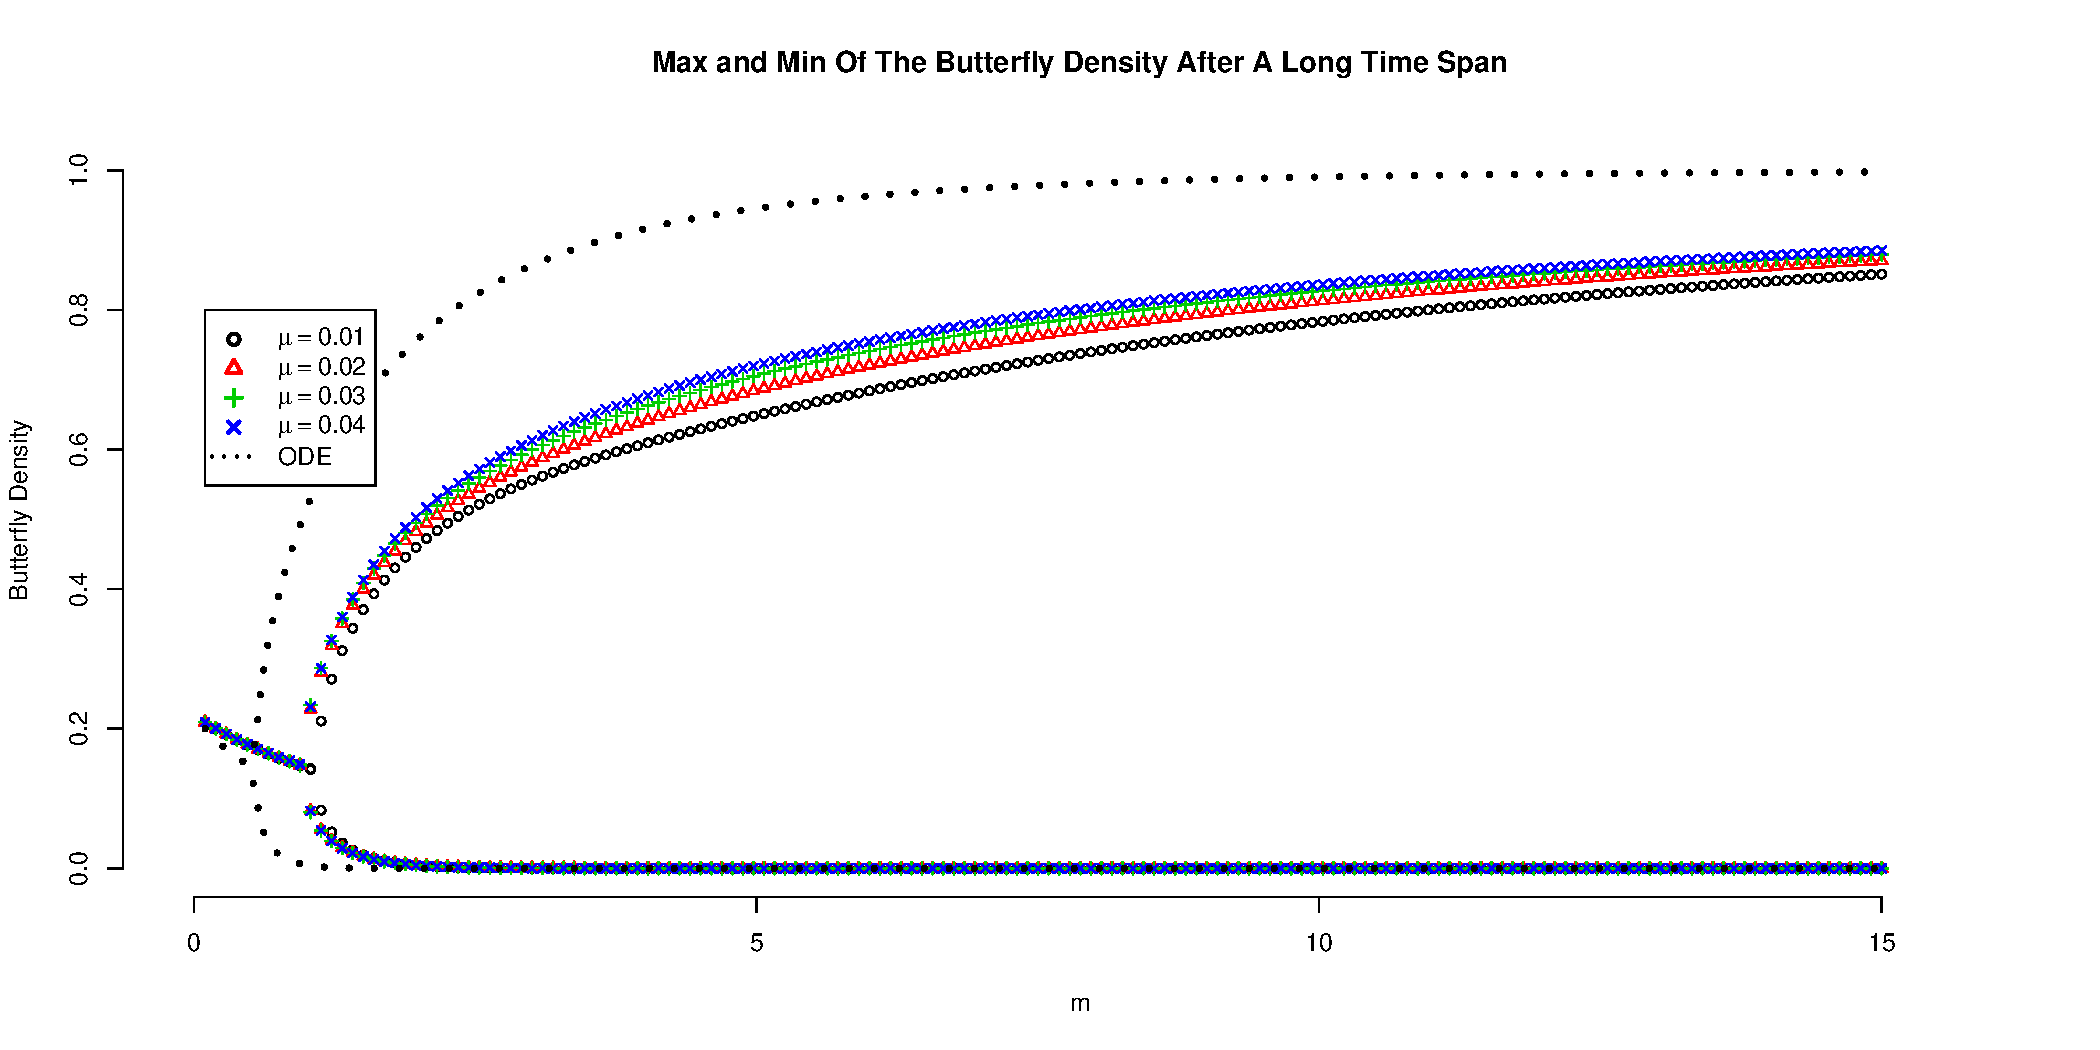
\includegraphics[height=8cm]{FIGURES/maxMinByM-c-1.1.pdf} 
  &
  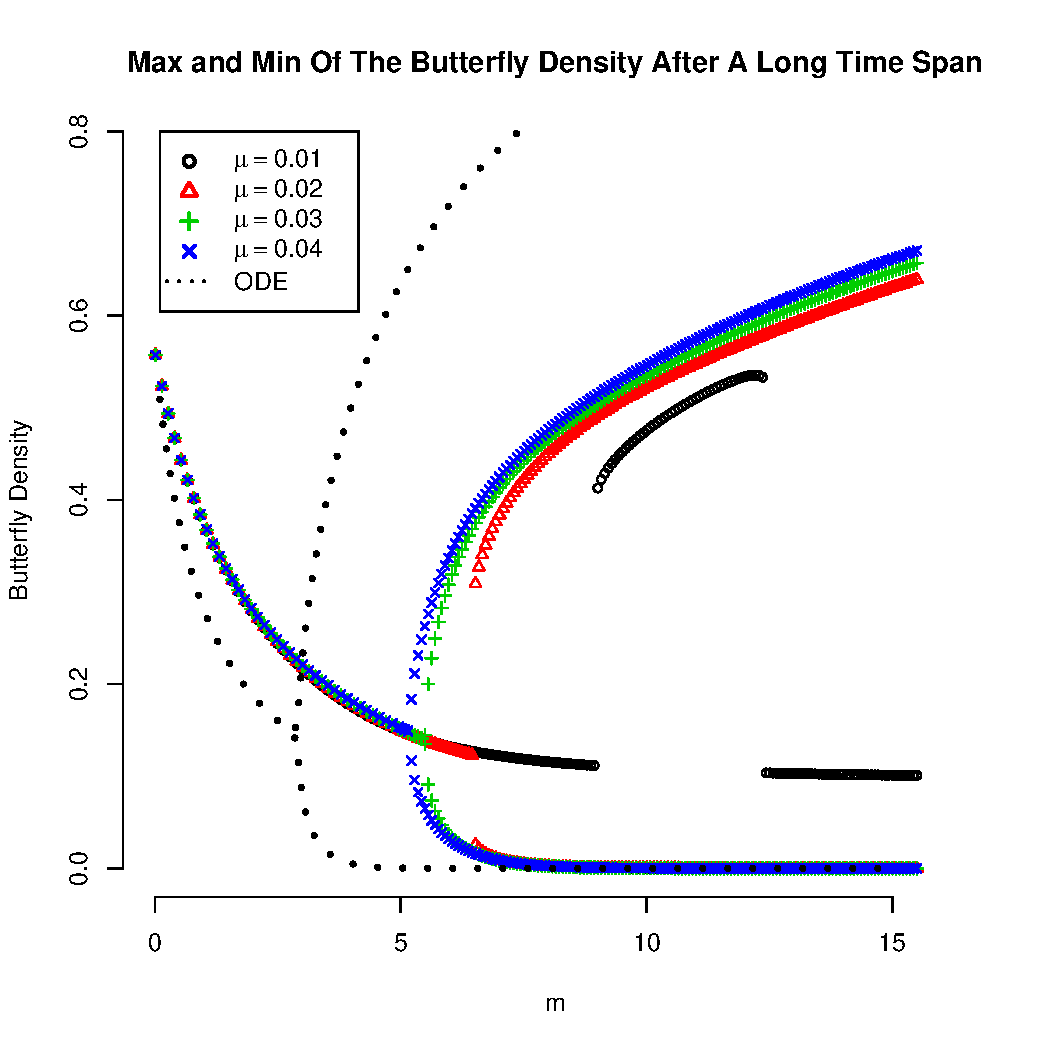
\includegraphics[height=8cm]{FIGURES/maxMinByM-mu-01-04.pdf} \\
  \multicolumn{1}{c}{(A)} & 
  \multicolumn{1}{c}{(B)} \\
  \end{tabular}
  \caption[Upper and lower bounds of the butterfly density.]{The upper
    and lower bounds of the long term density of the butterfly
    population. Graph (A) represents the maximum and minimum values of limit cycles for $c=1.1$. Graph (B) represents the maximum and minimum values of the limit cycles for $c=2.8$. The population was approximated for different values
    of $m$. The approximation was stopped if it either became close to
    a steady state or a limit cycle.  The value of $g$ is 0.6, $d$ is 0.1. }
  \label{fig:odeButterflyMaxMin}
\end{figure}

\begin{figure}[htb]
  \begin{tabular}{p{0.5\textwidth}p{0.5\textwidth}}
  \includegraphics[height=8cm]{FIGURES/maxMinByM-c-1.1-mu-01-04.pdf} 
  &
  \includegraphics[height=8cm]{FIGURES/maxMinByM-c-2.8-mu-01-04.pdf} \\
  \multicolumn{1}{c}{(A)} & 
  \multicolumn{1}{c}{(B)} \\
  \end{tabular}
  \caption[Upper and lower bounds of the butterfly density.]{The  upper
    % https://www.overleaf.com/project/5eb9da10e929ab0001816b1e
    and lower bounds of the long term density of the butterfly
    population. The dashed line is the bounds for the ODE model, and the symbols are for the PDE model with different values of the diffusion parameter. The population was approximated for different values
    of $m$. The approximation was stopped if it either became close to
    a steady state or a limit cycle.  The value of $g$ is 0.6, $d$ is 0.1. The value of $c$ for the graph on the left (A) is 1.1, and the value of $c$ for the graph on the right (B) is 2.8.}
  \label{fig:odepdeButterflyMaxMin}
\end{figure}






\subsection{Numerical results for the system of ODEs}
\label{subsection:odeApproximation}

We now turn to examine the results of a numerical exploration of the solutions to 
equations (\ref{eq:scaledODE1}) and (\ref{eq:scaledODE2}).
We focus on the long term behaviour of the solutions to the 
system to determine whether the approximation results in movement toward a fixed point or
the existence of a limit cycle.


The long term behaviour for one parameter range is shown in Figure
\ref{fig:odeButterflyMaxMin} (see section \ref{numericalApproximationODE} for details on the numerical approximation).  
Our focus is on the behaviour of the solutions over different values of the parameter $m$, and explore the role that 
different values of $c$ play in the transitions between a stable fixed point versus a limit cycle. 
The values of the parameters in the example are
$g=0.6$, $d=0.1$. Approximations were constructed for values
of $m$ starting at $m=0.1$ and ending at $m=15.0$.  Graph (A) represents the maximum and minimum values of the limit cycles for $c=1.1$, and graph (B) represents the maximum and minimum values of the limit cycles for $c=2.8$. The impact of increasing the value of $c$ is to shift to a smaller value of $m$ where limit cycles first appear.

It is important to note that shortly after the transition from a stable to an unstable fixed point, the approximations of the limit cycle indicate the butterfly population moves very close to zero. This can be seen in Figure \ref{fig:odeButterflyMaxMin} where the extremes of the limit cycle are shown.

For the graph on the left in Figure \ref{fig:odeButterflyMaxMin}, $c=1.1$, the transition from a linearly stable fixed point to periodic solutions should occur at $m\approx 0.54$. With respect to the approximation that transition occurs near $m\approx ?$. For the graph on the right, for the graph on the right, $c=2.8$, the transition from a linear stable fixed point to periodic solutions should occur at $m\approx 2.92$. With respect to the approximation the transition occurs at $m\approx ?$. In general, that transition occurs at
\begin{eqnarray}
m^* & = & c - 1 + 2 u.
\end{eqnarray}
As $c$ increases the transition should occur at a larger value of $m$.





The value of $\theta$ is fixed at 1 for these approximations, and the Hopf bifurcation occurs at $m=2.92$. With respect to the numerical approximations, the system moved close to a steady state for values of $m$ less than about 2.841. For larger values of $m$ the system approached a limit
cycle. The resulting numerical simulations provide a close estimate of the location of the bifurcation.

\subsection{Numerical Results for the coupled PDE and ODE system}
\label{subsection:pdeApproximation}

In this subsection we provide a  numerical exploration of the full, coupled system of the PDE and
ODE, equations (\ref{eq:scaledodePDE1}) and (\ref{eq:scaledodePDE2}). The details of the full approximation method are
described in appendix \ref{numericalApproximation}. The parameter
range is similar to that in subsection
\ref{subsection:odeApproximation}. When comparing these results to the ODE model, it is important to note how the full population of the butterflies impact the dynamics. The PDE model may include a subset of the butterfly population whose predicted behaviour is to settle into a constant equilibrium as well as a subset of the butterfly population whose predicted behaviour is a limit cycle. The result is the onset for the transition to a limit cycle is delayed or no longer present.

The approximation for the first example examined is shown in Figure \ref{fig:approximationM12Mu01}. 
The value of the parameters in the example are $c=2.8$, $g=0.6$,
$d=0.1$, and $\mu=0.01$. The temporal behaviour of the system is
similar to that found in the previous subsection
\ref{subsection:odeApproximation}. For example, an approximation for
--- provide example for $m=5$. --- Need to discuss this.

The onset of a limit cycle is delayed with respect to the system of
ODEs. In particular, we compare how the behaviors between the ODE and PDE systems differ for different values of the parameter $m$, which controls the slope of the propensity function $p(\theta)$, in effect magnifying the way the behavior is expressed as well as the range of the propensity function (sensitivity to $\theta)$. In this way, higher $m$ values correspond to larger differences in the manifestation of the trait within a population. In the ODE system, there is no dependence on $\theta$, therefore choosing a particular value of $m$ corresponds to keeping the propensity for the use of anti-aphrodisiac fixed for the entire population. We note that when compared to the ODE system, it takes a larger value of $m$ for the system to settle into a periodic behavior, which is the less ideal state for the population given that the population may come close to zero, therefore making extinction more likely (see Figure \ref{fig:odepdeButterflyMaxMin}) in the presence of fluctuations due to external influences. The ecological implication of this may be that in the absence of variation, for a particular propensity for the use of anti-aphrodisiac, the population will be more likely to be destabilized, while in the presence of variation, the population will more likely remain at a constant equilibrium, which is more advantageous overall. 
\par Further, we also investigate how these results change as we vary the diffusion coefficient $\mu$ in the PDE system, which represents the rate at which the change in the group phenotype composition happens from generation to generation (for high values of $\mu$, the population becomes more well-mixed faster) (insert figure demonstrating impact of $\mu$ on the population). In this case, we compare how diffusion ($\mu$) impacts the population with various levels of variation in the manifestation of the trait ($m$). We see that when the group phenotype composition changes slowly ($\mu$ is relatively small, and distribution of the trait doesn't change rapidly), the population can have a larger variation in the manifestation of trait (higher values of $m$) and still be sustained (see Figure \ref{fig:odepdeButterflyMaxMin}). For larger values of $\mu$, the population would need to have less variation in the manifestation of the trait in order to be sustained. We also note that as $\mu$ gets large, the results start to resemble those of the ODE system with an increases in the use of anti-aphrodisiac resulting in the destabilization of the population. This is expected as faster changes in the group phenotype composition lead to a more well-mixed population and therefore should resemble the ODE system. In other words, the distribution of the population is relatively uniform with respect to $\theta$, therefore resembling the case of the ODE system where there is no dependence on $\theta$. Higher diffusion allows certain subsets of the populations to be mixed more rapidly. If a rapid fluctuation begins in one part of the distribution a higher diffusion will more rapidly distribute the population throughout the entire domain. A smaller diffusion will allow a rapid change  in one part of the distribution to propagate.
Spatially explicit population models tend to be more stable, with less tendency for extinction, compared to ODE models that exclude animal movement. Allowing individuals an opportunity to seek refuge is one reason enhancing stability. Similarly, implementing explicit variation for group phenotype composition appears to have an analogous effect on stability. 

\begin{figure}[htb]
  \centering
  \includegraphics[trim=5 12 5 5,clip,scale=0.7]{FIGURES/M_vs_Mu.pdf}
  \caption[$\mu$ vs m comparison]{Numerical simulations for low and high values of $\mu$ and $m$. For a fixed value of the parameter $\mu$, the tuning of parameter $m$ controls the impact associated with the use of anti-pheromone with higher values of m implying greater degree of variation within the butterfly population. For a fixed value of parameter $m$, we see that the impact of increasing the diffusion coefficient $\mu$ results in a more well mixed population, with the expression level becoming more evenly distributed within the population. For all simulations, we looked at the time corresponding to the maximum peak in the $\theta$ distribution and plotted the butterfly densities across all $\theta$s for that specific time point.}
  \label{fig:mu_vs_m}
\end{figure}
 Include interpretation for c: the parameter c dictates the rate of saturation.  We note that the previous result discussed is exaggerated for higher values of c.     For $m=5$ the fixed point for the ODEs results in a
limit cycle. However, in the case of the coupled PDE and ODE system a
limit cycle did not appear until much larger values of $m$. For
example, at $m=12$, a repeating pattern was found. The results of an
approximation are shown in Figure \ref{fig:approximationM12Mu01}.

The results shown in Figure \ref{fig:approximationM12Mu01} are only
for a short time span in order to make it easier to show the change in
time. A question arises is the importance of the initial condition, and various initial conditions were examined all of which resulted in similar outcomes. For example, the initial condition in this case is a Gaussian function with a center
at the right end point of the domain consistent with a scenario in which the majority of the population exhibits a higher propensity for using the pheromone.  Similar patterns emerge for an initial
condition that is a Gaussian centered at the left characterizing a scenario in which the population exhibits a lower propensity for using the pheromone, a constant initial
condition, and an initial condition with the butterfly density set at
the theoretical steady state given each value of $\theta$.

To compare the impact of the parameter $m$, a similar approximation was
constructed with the same values for the parameter, except that $m=15$. 
The results are shown in Figure \ref{fig:approximationM15Mu01}. In this 
case there are some initial oscillations in the populations, but the 
changes rapidly move to a steady state.

Approximations were constructed for
values of $m$ sarting at $m=0.1$ and ending at $m=15.0$.


\begin{figure}[htb]
  \centering
  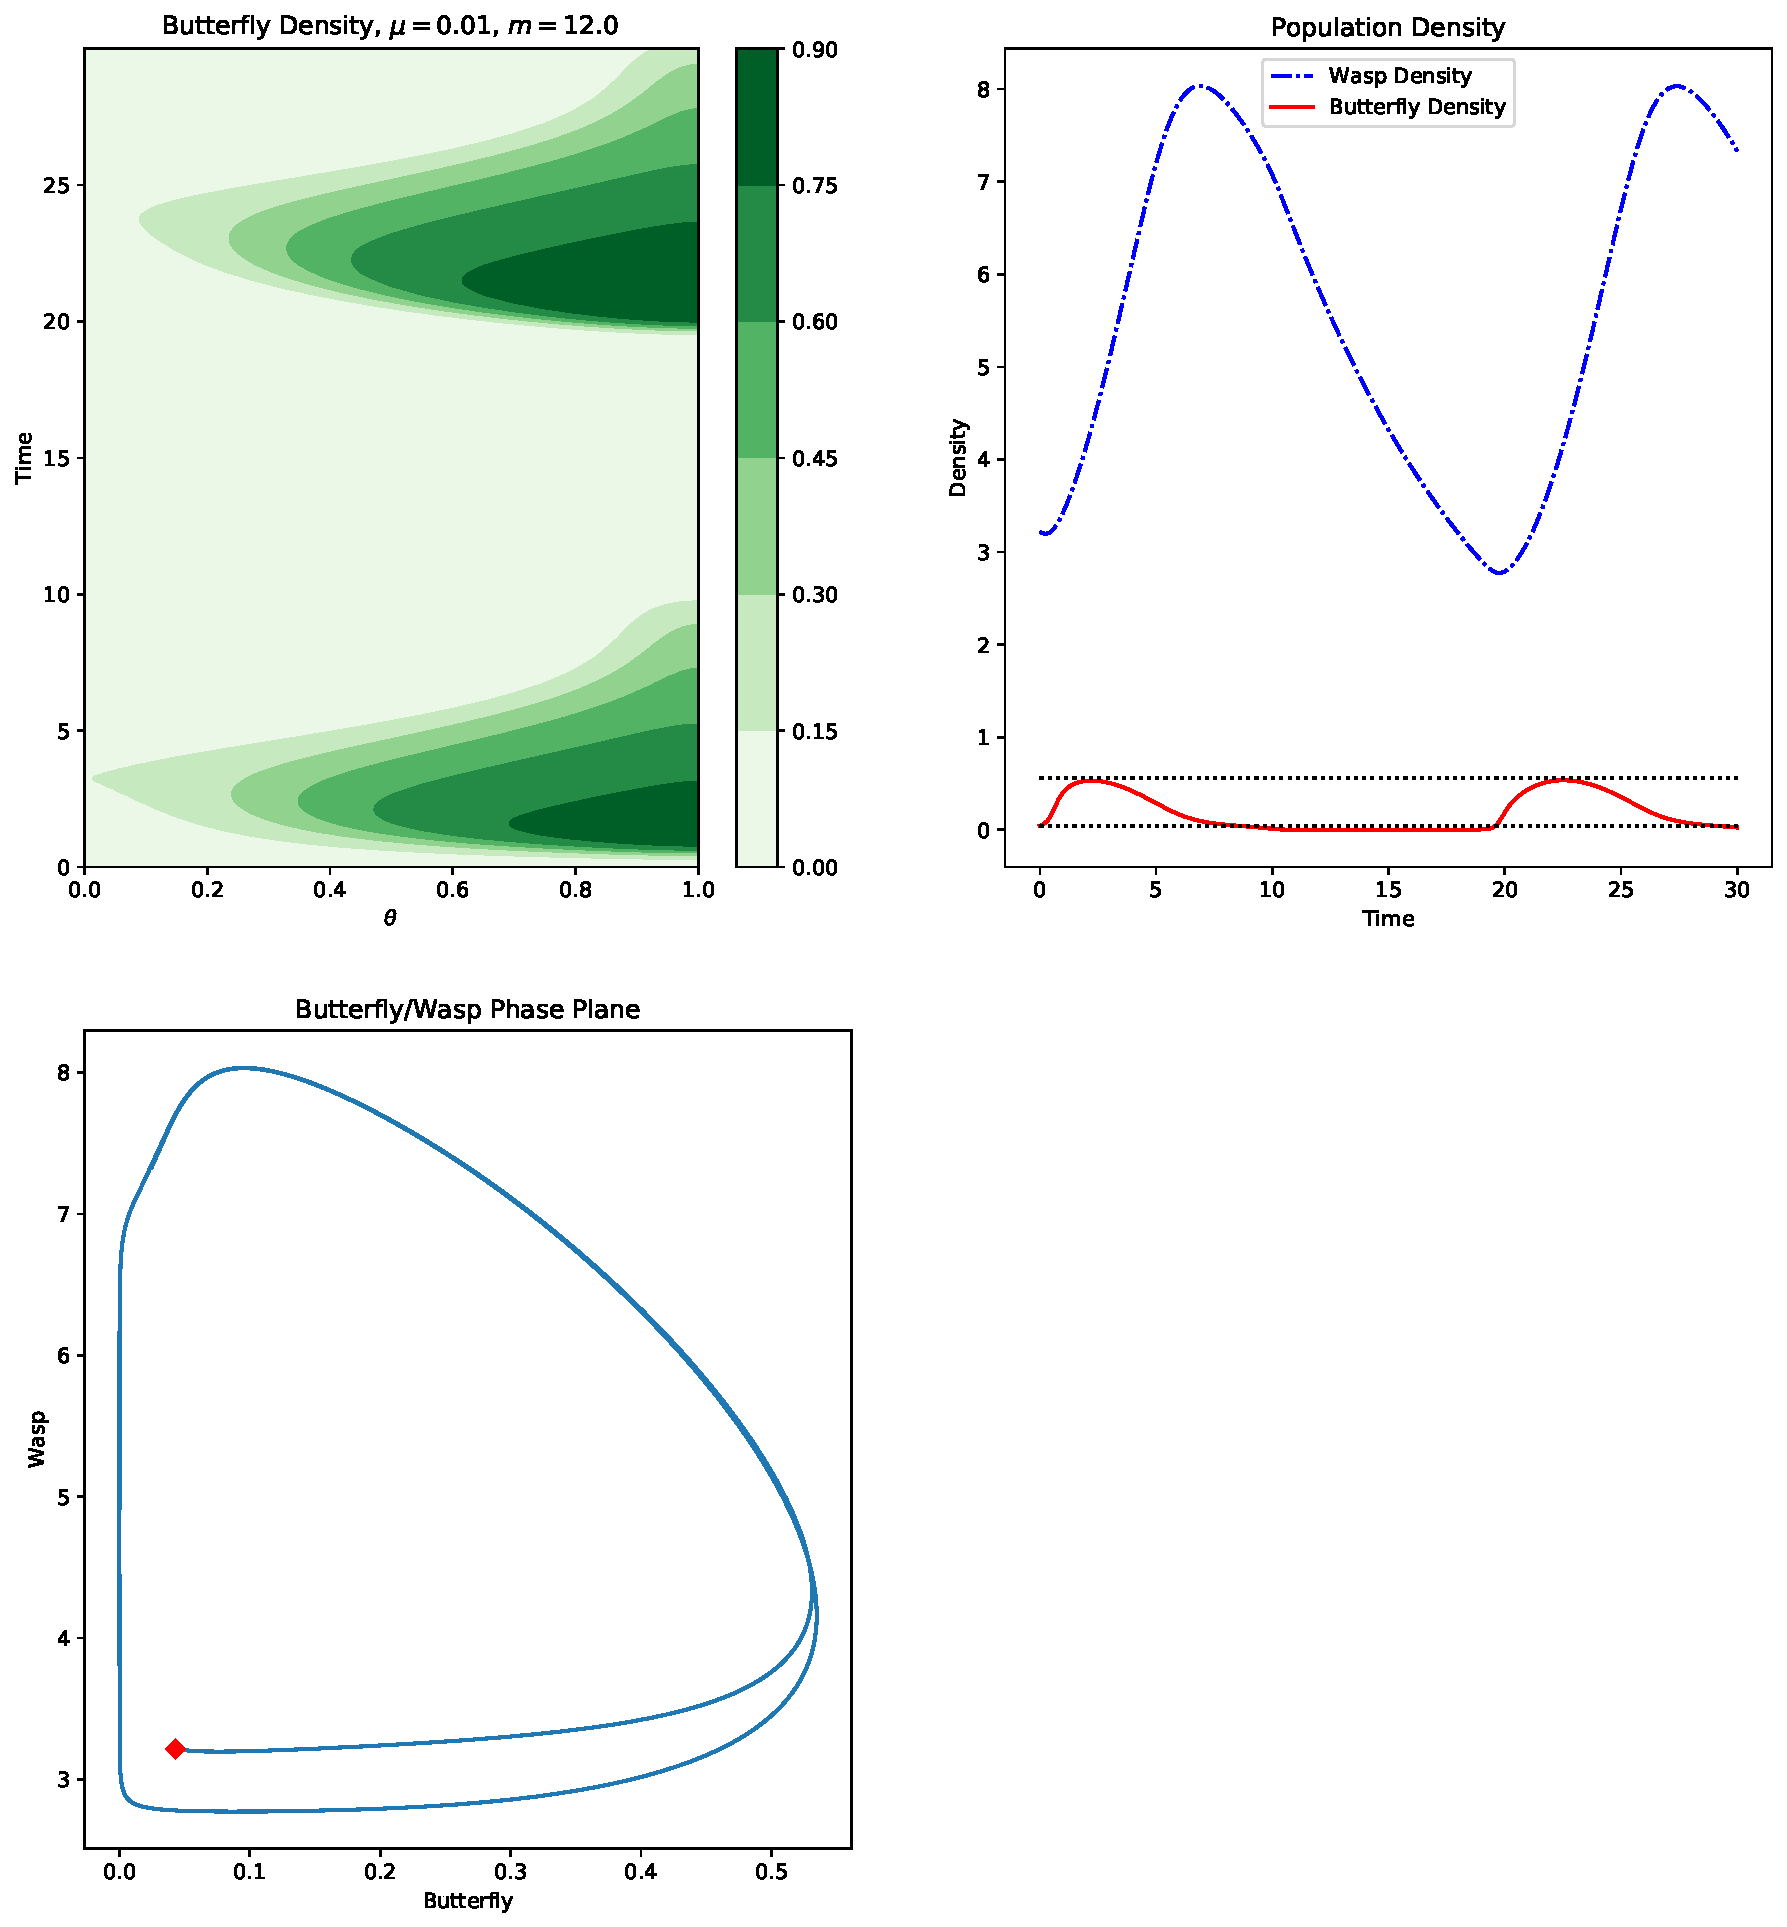
\includegraphics[width=12cm]{FIGURES/approximation-mu-01-m-12.pdf}
  \caption[Approximation with $m=12$ and $\mu=0.01$.]{Approximation of
    the system, $m=12$, $\mu=0.01$, $c=2.8$, $g=0.6$, and $d=0.1$. }
  \label{fig:approximationM12Mu01}
\end{figure}

\begin{figure}[htb]
  \centering
  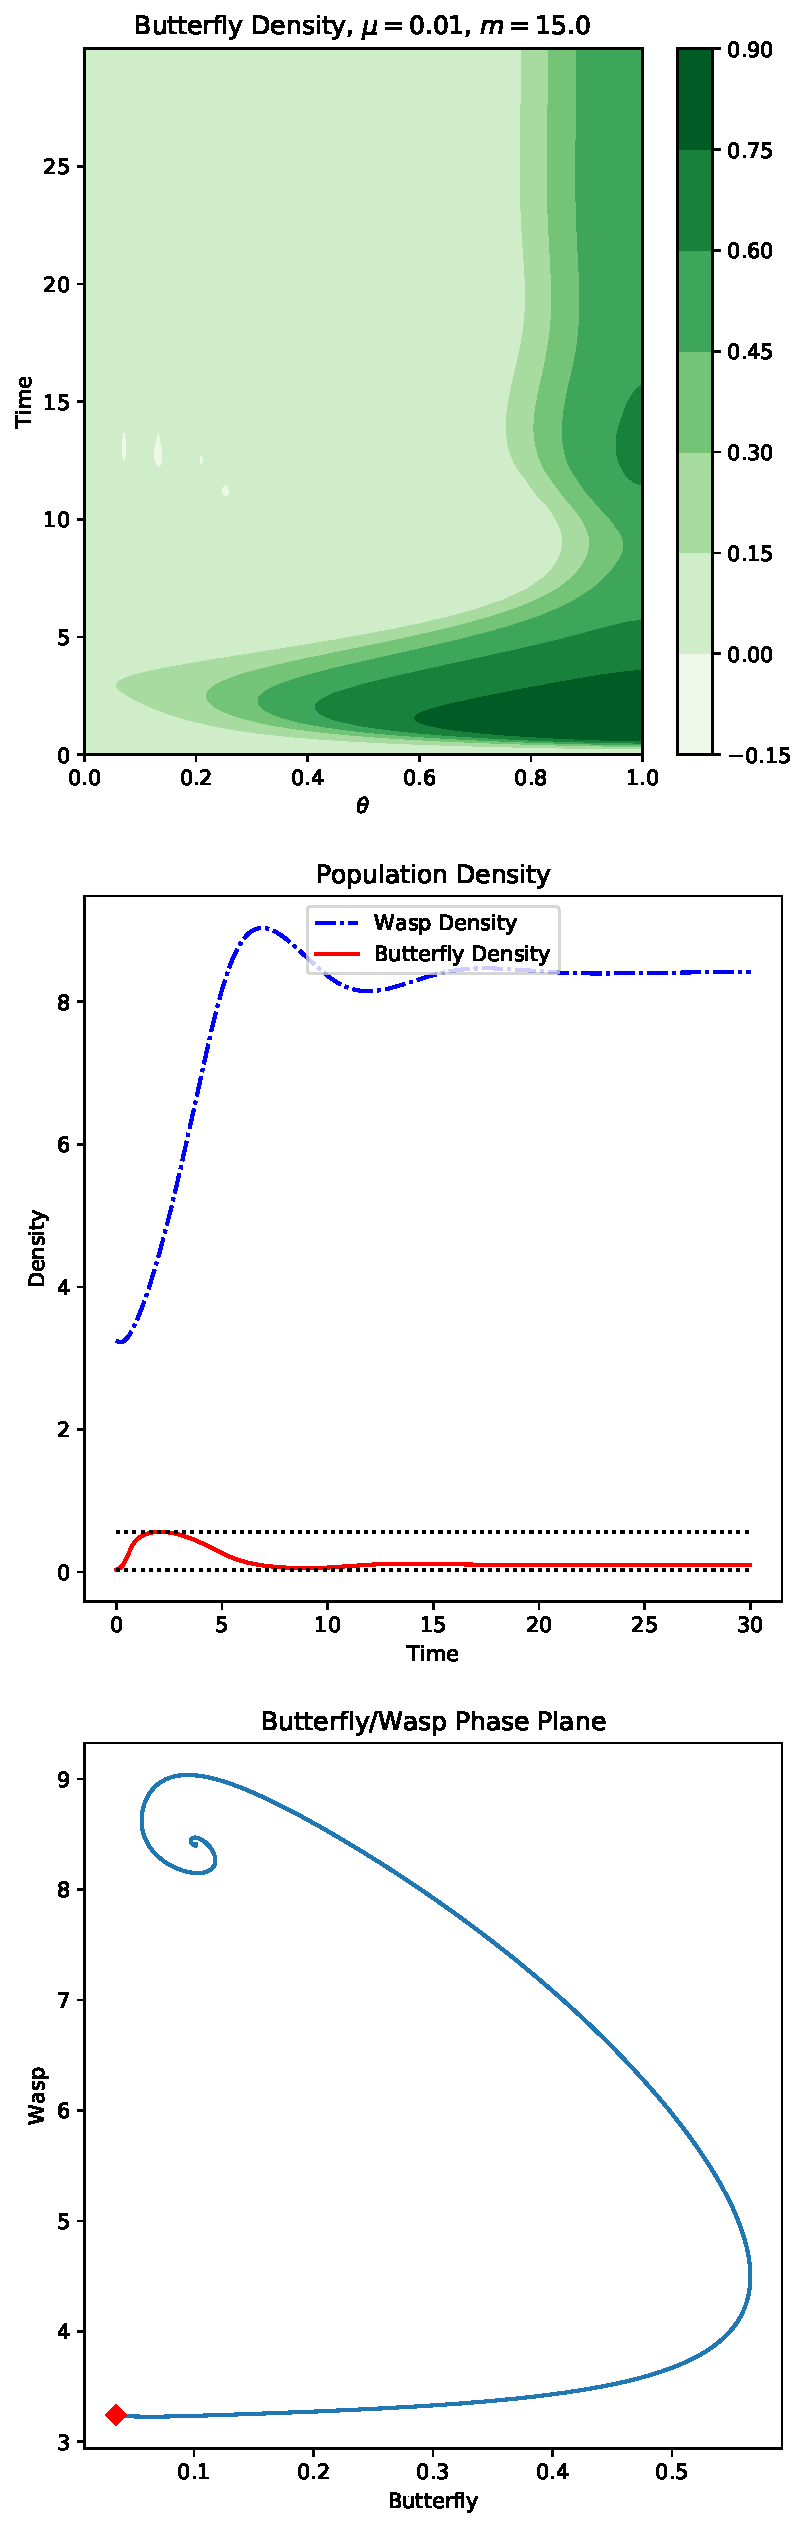
\includegraphics[width=12cm]{FIGURES/approximation-mu-01-m-15.pdf}
  \caption[Approximation with $m=15$ and $\mu=0.01$.]{Approximation of
    the system, $m=15$, $\mu=0.01$, $c=2.8$, $g=0.6$, and $d=0.1$. }
  \label{fig:approximationM15Mu01}
\end{figure}

Figure \ref{fig:approximationM01Mu01C11} Approximation of
the system, $m=0.01$, $\mu=0.01$, $c=1.1$, $g=0.6$, and $d=0.1$.  
In this example we get rapid convergence to a steady state. The value of $m$ is small. In Figure \ref{fig:approximationM51Mu01C11} we increase $m$ to 0.51. 
Goes to steady state but slowly oscillates to the steady state.
In Figure \ref{fig:approximationM150Mu01C11} increase $m$ to 1.5.
Now see oscillations.

\begin{figure}[htb]
  \centering
  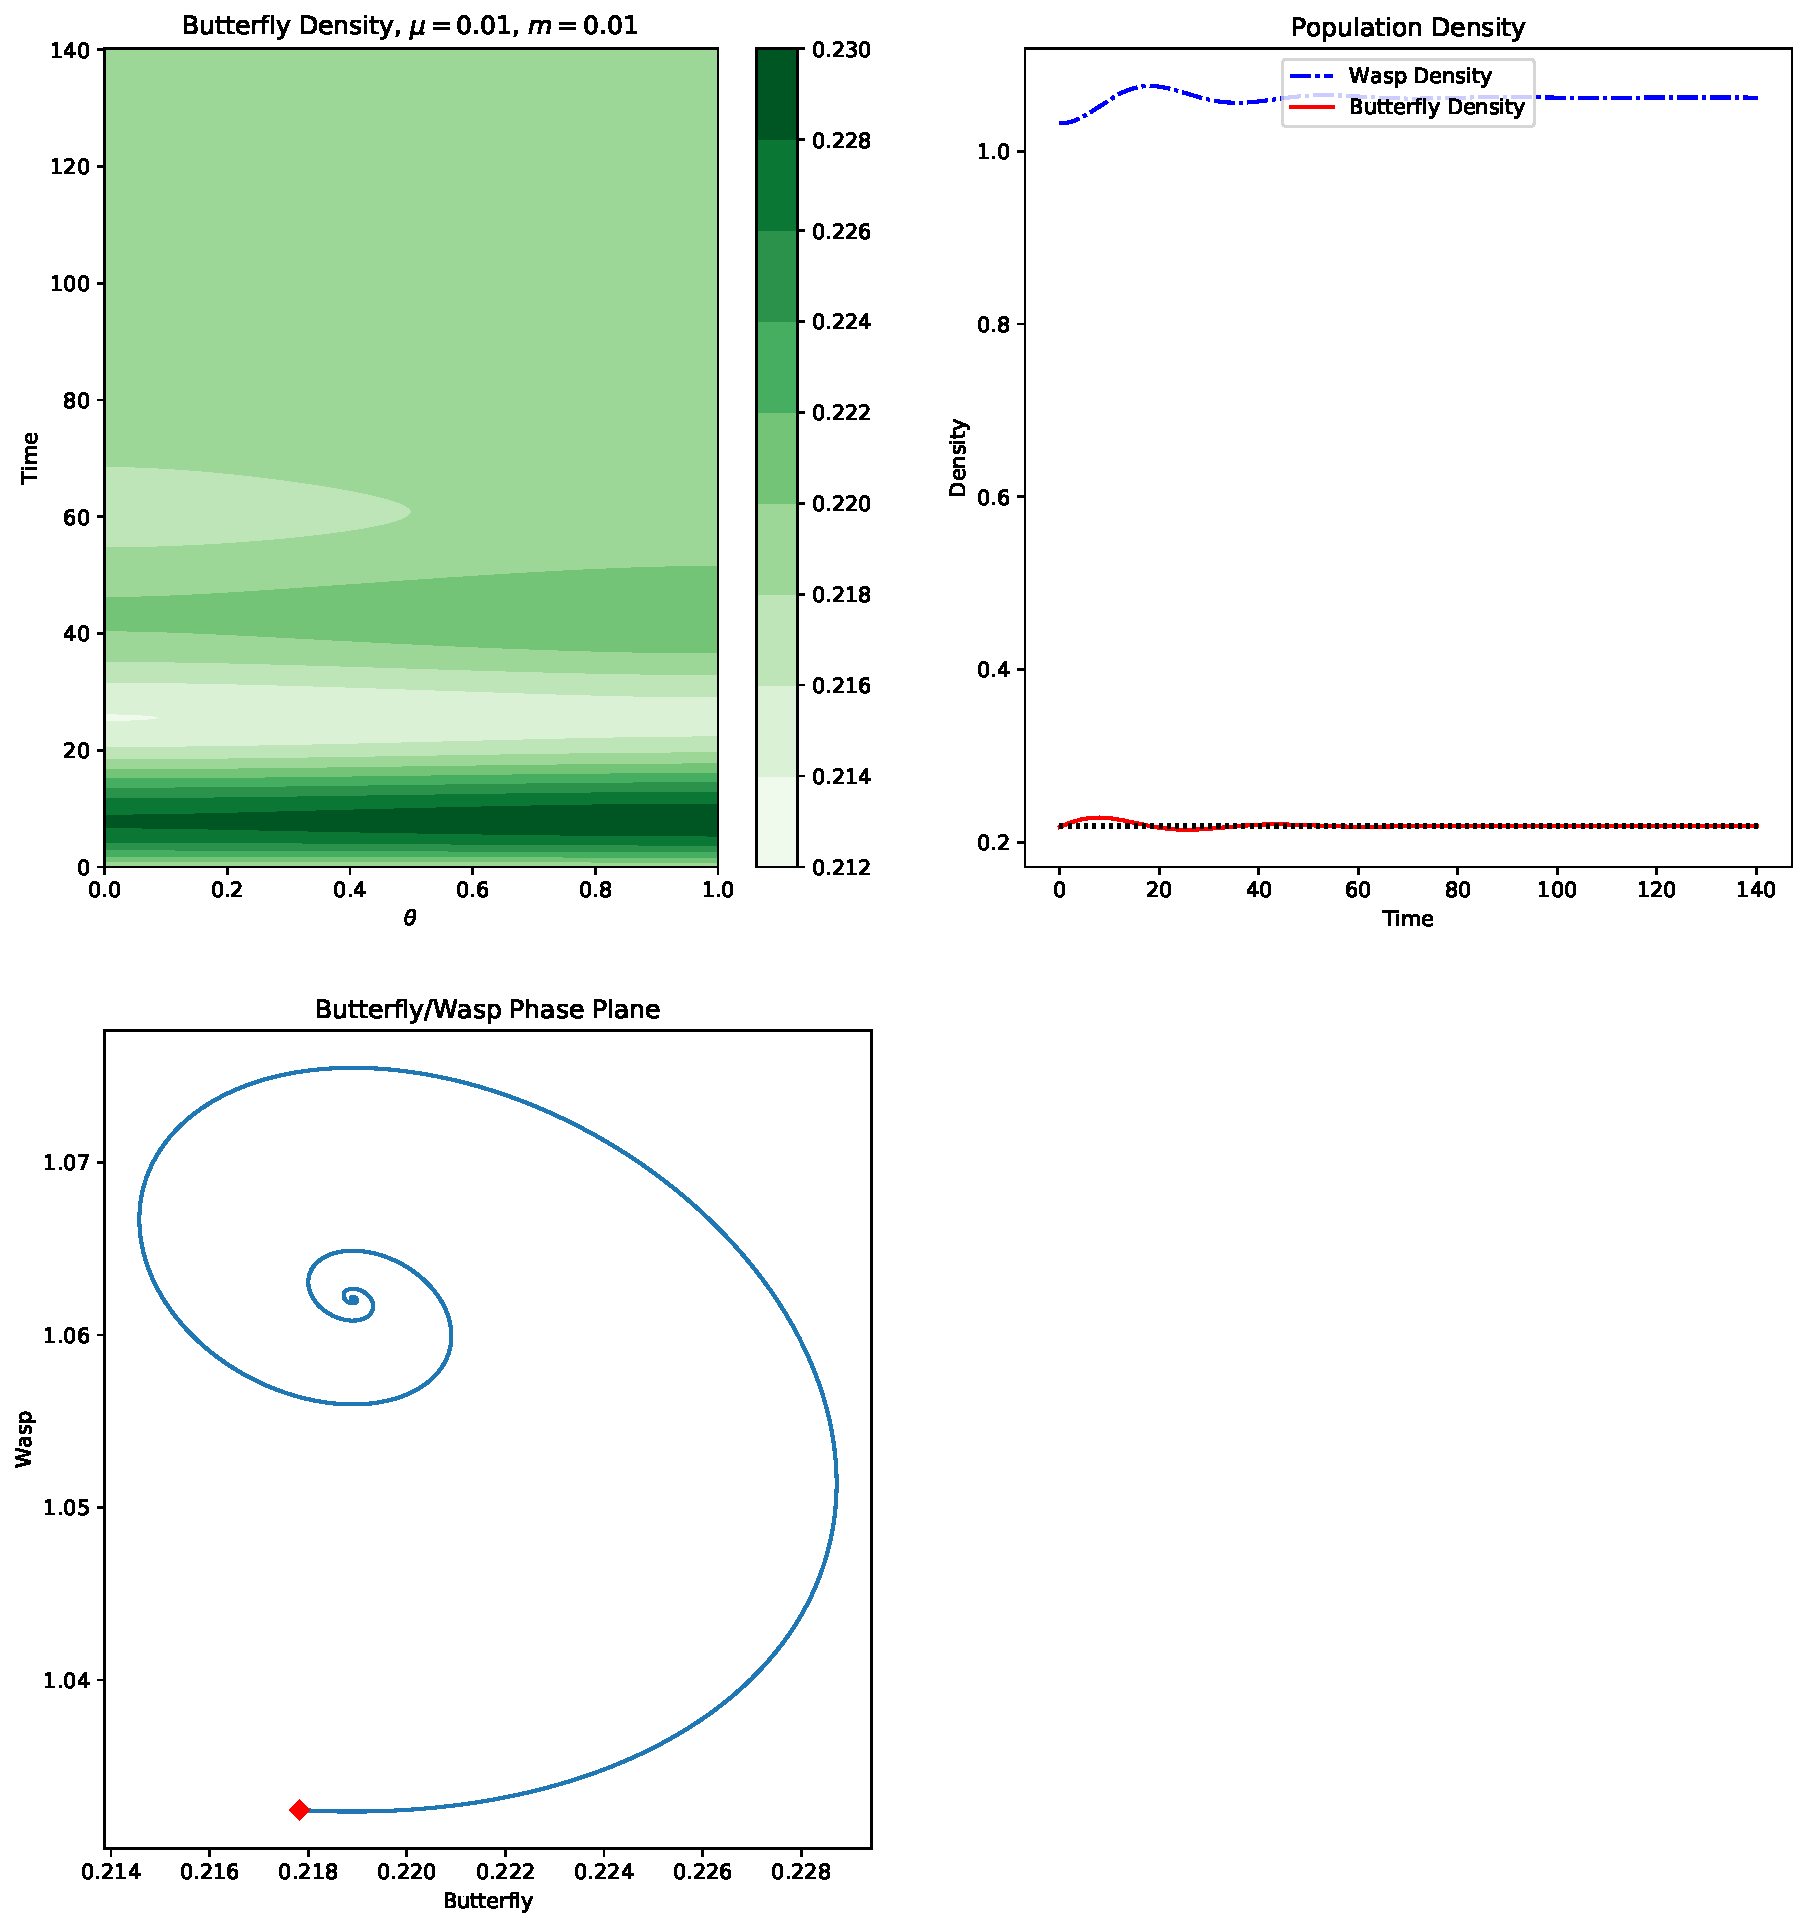
\includegraphics[width=12cm]{FIGURES/approximation-c-11-mu-01-m-01.pdf}
  \caption[Approximation with $c=1.1$, $m=0.01$ and $\mu=0.01$.]{Approximation of
    the system, $m=0.01$, $\mu=0.01$, $c=1.1$, $g=0.6$, and $d=0.1$. }
  \label{fig:approximationM01Mu01C11}
\end{figure}

\begin{figure}[htb]
  \centering
  \includegraphics[width=12cm]{FIGURES/approximation-c-11-mu-01-m-51.pdf}
  \caption[Approximation with $c=1.1$, $m=0.51$ and $\mu=0.01$.]{Approximation of
    the system, $m=0.51$, $\mu=0.01$, $c=1.1$, $g=0.6$, and $d=0.1$. }
  \label{fig:approximationM51Mu01C11}
\end{figure}


\begin{figure}[htb]
  \centering
  \includegraphics[width=12cm]{FIGURES/approximation-c-11-mu-01-m-150.pdf}
  \caption[Approximation with $c=1.1$, $m=1.50$ and $\mu=0.01$.]{Approximation of
    the system, $m=1.50$, $\mu=0.01$, $c=1.1$, $g=0.6$, and $d=0.1$. }
  \label{fig:approximationM150Mu01C11}
\end{figure}



\begin{figure}[!htp]
\begin{center}
\includegraphics[scale=0.6]{FIGURES/Simulations_mu_0.04.eps} 
\includegraphics[scale=0.2]{FIGURES/Ratio_mu0.01.jpg}  
\end{center}

\caption{Figure A shows a selection of runs in the $m-c$ parameter space for $\mu=0.04$. Figure B shows the $m-c$ parameter space for $\mu=0.01$. Low values of c correspond to a high-predation scenario, where wasps receive the most benefit from butterfly consumption. The parameter $m$ corresponds to the variation of the trait manifestation within the butterfly population. Some things to note: 1) In the presence of higher variation of the trait in the butterfly population, the "strong" survive at the expense of the weak (the level of predation still plays a role here, too).
2) The oscillations of the wasp population get close to zero in the low-c region. This may be due to the length of the cycle in the butterfly population (as compared to the scenario in the higher-c region). The wasps don't have enough time to recover from a rapid collapse of the butterfly population. 3) As $\mu$ decreases, the idea of "the strong" butterflies (those that display the trait, higher $\theta$)  surviving at the expense of the "weak" is more clearly observed. This should make sense as lower $\mu$ corresponds to less homogeneous populations, which remains so for longer (the trait distribution changes slowly from generation to generation) 4) May be worth exploring and framing in the context of "realistic" versus "ideal" region?
Details about the code:  Latin Hypercube Sampling is used to generate N sets of samples from the $m-c$ parameter space. For each pair of parameter values, I integrate the PDE using the explicit finite difference method. Considering only the second half of the time domain (to exclude possible transient behavior), I look at the 80th percentile of theta values and find the maximum butterfly density ($B_{high\theta}$). For the same value of $t$, I look at the 20th percentile of theta values and find the maximum butterfly density ($B_{low\theta}$). Finally, I compute the ratio $\frac{B_{high\theta}}{B_{low\theta}}$ and plot them on a color scale such that values below 1 are marked red, values close to 1 are marked green, and those that deviate significantly from 1 are colored using a grey scale.}
      \label{fig:mvsc}
\end{figure}

\section{Conclusion}

Need stuff here about the differences between our results and the Huigen's prediction of evolutionary pressure to be less likely to use the anti-aphrodisiac pheromone.

\section{Acknowledgements}

\clearpage

\appendix

\section{Stability analysis of the ODE system}
\label{appendix:otherFixedPoints}

In subsection \ref{subsection:parameters}, we examined the stability of the
non-trivial fixed point in the positive quadrant for the ODE system given by equations (\ref{eq:scaledODE1}) and
(\ref{eq:scaledODE2}). In this appendix we provide a more complete stability analysis for all fixed points of this system.  In particular  two other
fixed points are determined and the linear
stability at these two fixed points is discussed.

The  system of equations given in by
(\ref{eq:scaledODE1}) and (\ref{eq:scaledODE2}) has (at most) one fixed point
with both $b>0$ and $w>0$.  This was discussed in \ref{subsection:parameters} and given as $b^*= \frac{dc}{(g-d)p}$ and $w^* = (c+\frac{dc}{g-d})(1- \frac{dc}{(g-d)p}).$  There are two other fixed points on the boundary of the positive quadrant, i.e $b=0$ or $w=0$.  One is the fixed point at the origin, $b=0$ and $w=0$.
The remaining fixed point occurs at $b=1$ and $w=0$. 
  

The stability at these two fixed points can be examined by first
determining the Jacobian of the system,
\begin{eqnarray*}
  J & = & \left[
          \begin{array}{rr}
            J_{11} & J_{12} \\
            J_{21} & J_{22}
          \end{array}
          \right].
\end{eqnarray*}
The entries in the matrix are given by
\begin{eqnarray*}
  J_{11} & = & p(1-2b) -
               \frac{w  c   p}{\left( c + pb \right)^2}, \\
  J_{12} & = & -\frac{pb}{c+pb}, \\
  J_{21} & = & g \cdot\frac{wcp}{(c+pb)^2}, \\
  J_{22} & = & -d + g  \cdot \frac{pb}{c+pb}.
\end{eqnarray*}

For the fixed point at the origin, the Jacobian reduces to 
\begin{eqnarray*}
  J~\bigg|_{(0,0)} & = & \left[
          \begin{array}{rr}
            p & 0 \\
            0 & -d
          \end{array}
          \right].
\end{eqnarray*}
Since it is assumed that both $p$ and $d$ are non-negative, this fixed point  is unstable  (saddle point).



At the fixed point $b=1$, $w=0$, the Jacobian is given by 
\begin{eqnarray*}
  J~\bigg|_{(1,0)} & = & \left[
          \begin{array}{cc}
            -p & -\frac{p}{c+p} \\
            0 & -d+\frac{gp}{c+p}
          \end{array}
          \right].
\end{eqnarray*}

This fixed point is unstable as long as $p >\frac{dc}{g-d}$.  This condition is equivalent to $b^* < 1$.  (If on the other hand, $p <\frac{dc}{g-d}$, then the equilibrium $(b^*,w^*)$ moves into the fourth quadrant ($w^*<0$) and the equilibrium $(1,0)$ is a stable attractor.)


\noindent
\textbf{Limit Cycles}

In \ref{subsection:parameters} we showed that there is an equilibrium solution $(b^*,w^*)$ in the positive quadrant for the ODE system under the conditions:  1.)  $g-d>0$, and 2.) $\frac{cd}{g-d}<p$.   Here, the values of  $p$ are constrained by $1<p<1+m$.   We also showed in that section that this 
equilibrium is stable if and only if $\frac{p-c}{2} < \frac{cd}{g-d}.$   In this appendix, we prove the existence of a limit cycle when this latter inequality fails, i.e. the equilibrium becomes unstable.

We begin by remarking that the positive quadrant of the $(b,w)$-plane is invariant under the flow of the ODE system.

\begin{lemma}


All solutions of equations (\ref{eq:scaledODE1}) and
  (\ref{eq:scaledODE2}) with initial values
  $b\left( 0\right) > 0 ,w\left( 0\right) >0$ remain in the positive quadrant, $\mathbb R_+^2$, for all time.
\end{lemma}

\begin{proof}
  This follows by noticing that the non-negative axes, $\{(b,0):\  b \ge 0\}$ and $\{(0,w):\  w\ge 0\}$ are invariant under the flow, that is, if a solution starts in this set then it remains in this set. Then, by uniqueness, we conclude that no flow line can pass from the positive quadrant through these axes.
\end{proof}

We next show that all solutions in the positive quadrant are bounded for all positive time.  

\begin{lemma}
There exists $R_{0}>0$  such that for all $R\geq R_{0}$, the right
triangle, 
$$T_{R}=\left\{ \left(b,w\right) \in \mathbb R^{2}:\  b\ge 0, w\ge 0, \ {\rm and}\  b+\frac{1}{g}w\le R\right\}, $$  
is positively invariant.
\end{lemma}

\begin{proof}
  We first note that if for some $t_0$, $b(t_0)< 1,$ then $b(t) < 1$ for all $t>t_0$.  This follows from the fact that equation (\ref{eq:scaledODE1}) shows that 
  $$\frac{d}{dt}b(t) < 0,\  \  {\rm when}\ \ b(t)\ge 1.$$
  
  Now, since we have already discussed that solutions in the positive quadrant cannot cross the axes, it is only left to show that we can choose $R_0$ large enough so that if $R>R_0$, we have
  $$\frac{d}{dt}\left(b(t)+\frac{1}{g}w(t)\right) <0,\  {\rm when}\  b(t)+\frac{1}{g}w(t) =R.$$
  
  But from equations (\ref{eq:scaledODE1}) and (\ref{eq:scaledODE2}), we have
  $$\frac{d}{dt}\left(b(t)+\frac{1}{g}w(t)\right)  = p b(t)\left( 1-b(t)\right) -\frac{d}{g}
w\left( t\right) . $$

If $b(t) \ge 1$, the right hand side in negative.  On the other hand, if $b(t) < 1$, we use $\frac{d}{g}w(t) = d(R-b(t))$ to get
$$\frac{d}{dt}(b(t)+\frac{1}{g}w(t)) =p b(t)\left(
1-b(t)\right) -d\left( R-b(t)\right),$$
which is negative if $R>R_0= \frac{p}{d} +1.$
\end{proof}

Finally, applying the Poincair\'{e}--Bendixson theorem \citep{nonlinearChaos}, together with the above lemma, we have

\begin{theorem}
  If $0 < \frac{cd}{g-d} < \frac{p -c}{2}$, then there exists at least one  limit cycle solution to equations (\ref{eq:scaledODE1}) and (\ref{eq:scaledODE2}) in the positive quadrant.
\end{theorem}

Summarizing these results, we have

\begin{theorem}
  The system of ordinary differential equations given by equations (\ref{eq:scaledODE1}) and (\ref{eq:scaledODE2}) (with $g\ne d)$ has fixed points in the $(b,w)$-plane at the points $(0,0), (1,0),$ and $(b^*,w^*)$, where $b^*=\frac{cd}{p(g-d)}$ and
$w^*=\left(\frac{cd}{g-d}+c\right)\left(1-\frac{cd}{p(g-d)}\right)$. 
 The  fixed point $(b^*,w^*)$ lies in the positive quadrant if $g-d>0$ and $u<p$, where $u=\frac{cd}{g-d}.$ Considering $u$ as a bifurcation parameter, the system undergoes a Hopf bifurcation at $u^* = \frac{p-c}{2}$.  
That is, the fixed point $(b^*,w^*)$ is asymptotically stable when $u>\frac{p-c}{2}$ and is unstable if $u<\frac{p-c}{2},$ and, since all positive solutions to the system are bounded,  there is at a  limit cycle in the positive quadrant when the fixed point is unstable.
Finally, the fixed point $(0,0)$ is always an unstable saddle point, and the fixed point $(1,0)$ is unstable when $u<p$, otherwise it is stable.
\end{theorem}

%\section{Stability of the %Equilibria}
\label{appendix:stability}


\iffalse

The linear stability with respect to the parameters for the
non-trivial fixed points is examined in subsection 
\ref{subsection:parameters}. We now turn our attention to the
existence of limit cycles or oscillatory behaviour of the solutions
near the equilbria. Consider the model system, equations
(\ref{eq:scaledODE1}) and (\ref{eq:scaledODE2}). Can the impact
associated with the use of the anti-pheromone destabilize/stabilize
this equilibrium? If so, under what conditions? This is settled via
the following lemma,
\begin{theorem}
  \bigskip\ All solutions of equations (\ref{eq:scaledODE1}) and
  (\ref{eq:scaledODE2}) with initial values
  $b\left( 0\right) ,w\left( 0\right) >0$ are always non-negative
\end{theorem}


\begin{proof}
  Notice that equations (\ref{eq:scaledODE1}) and
  (\ref{eq:scaledODE2}) have the form
\begin{eqnarray}
  b^{\prime}\left( t \right) & = & b(t)X\left( b,w\right), \\
  w^{\prime}\left( t \right) & = & w(t)Y\left( b,w\right).
\end{eqnarray}


If $\ \left( b\left( t\right) ,w\left( t\right) \right)
$ is a solution of such a system, then using an integrating factor
\begin{eqnarray}
\dfrac{d}{dt}\left( e^{\left( -\int_{0}^{t}X(s)ds\right) }b(t)\right) & = & 0
\end{eqnarray}
Consequently,
\begin{eqnarray}
b(t) & = & e^{\left( -\int_{0}^{t}X(s)ds\right) }b(0), \\
w(t) & = & e^{\left( -\int_{0}^{t}Y(s)ds\right) }w(0).
\end{eqnarray}
So for all $t>0$ and $b\left( 0\right) ,w\left( 0\right) >0$ .
\end{proof}

Having established that the solutions are non-negative our attention
now turns to whether or not the solutions are bounded. We can state
that the solutions are bounded in the first quadrant.
\begin{lemma} \label{mm}
All the solutions of the system (\ref{eq:scaledODE1}) and (\ref{eq:scaledODE2}) which start in $R_{+}^{2}$ are
uniformly bounded. Furthermore There exists $R_{0}>0$  such that for all $R\geq R_{0}$, the right
triangle $T_{R}$ with sides $b=0, w=0$ and $R=b+\frac{1}{g}w $ is positively invariant.
\end{lemma}

\begin{proof}
For all $R>0$, consider the triangular regions $T_{R}=\left\{ \left(b(t),w(t)\right) \in R_{+}^{2}:R=b+\frac{1}{g}w\right\} $\\
Let's assume that $b(t),w(t)$ are any positive solution of system (\ref{eq:scaledODE1}) and (\ref{eq:scaledODE2}),
then it is obvious that

$$\frac{d}{dt}b(t)\leq \hat{p}\left( \theta \right) b(t)\left( 1-b(t)\right) $$

We can see from the comparison argument that

$$0\leq b(t)\leq 1$$
Now since every initial point $b(0),w(0)\in R^{+}$ satisfies $b(0),w(0)\in T_{R}$ for some $R\geq R_{0}$, this shows that all solutions starting in $R^{+}$ are bounded for $t\geq 0$.\\
We claim that $T_{R}$ is forward invariant for all sufficiently large $R.$ We
need only to show that solutions cannot leave $T_{R}$\\
Since $R=b+\frac{1}{g}w $, 
it is enough to show that $\frac{d}{dt}\left( b(t)+\frac{1}{g}w(t)\right)\geq 0$

$$\frac{d}{dt}\left( b(t)+\frac{1}{g}w(t)\right)
=\left( \hat{p}\left( \theta \right) b(t)\left( 1-b(t)\right) -\frac{d}{g}%
w\left( t\right) \right) $$

$$ =\hat{p}\left( \theta \right) b(t)\left(
1-b(t)\right) -d\left( R-b(t)\right) \leq 0$$

if $R$ is chosen large enough.
\end{proof}

\begin{theorem}
  \index{3} Consider the model equations (\ref{eq:scaledODE1}) and
  (\ref{eq:scaledODE2}). Assume that  $g>d$.
 
\end{theorem}

\begin{description}
\item[1]  If $%
p(\theta )=c+\dfrac{2cd}{g-d},$ then the non trivial equilibrium $%
E^{\ast }=(b^{\ast },w^{\ast })$ is center.

\item[2] If $0<p(\theta )<c+\dfrac{2cd}{g-d}$ then the non trivial
equilibrium $E^{\ast }=(b^{\ast },w^{\ast })$ is locally stable.
\end{description}

\begin{proof}
  The non trivial equilibrium $E^{\ast }=(b^{\ast },w^{\ast })$ of the
  model equations (\ref{eq:scaledODE1}) and (\ref{eq:scaledODE2}) will
  be center if $DetJ>0$ and $TraceJ=0$

since $DetJ>0$ all the time then the it only depend on the value of the $%
TraceJ$
\begin{center}
$TraceJ=J_{11}=00$

iff $p(\theta )b^{\ast }\left( -1+\dfrac{p(\theta )w^{\ast }}{%
\left( c+p(\theta )b^{\ast }\right) ^{2}}\right) =0$

iff $p(\theta )w^{\ast }=\left( c+p(\theta )b^{\ast }\right)
^{2} $

iff $p(\theta )\left( 1-b^{\ast }\right) =\left( c+p(\theta
)b^{\ast }\right) $

iff $p(\theta )-2p(\theta )b^{\ast }=c$

iff $p(\theta )-\dfrac{2cd}{g-d}=c$

if $p(\theta )=c+\dfrac{2cd}{g-d}$
\end{center}

\end{proof}
\begin{figure}[!htp]
\begin{center}
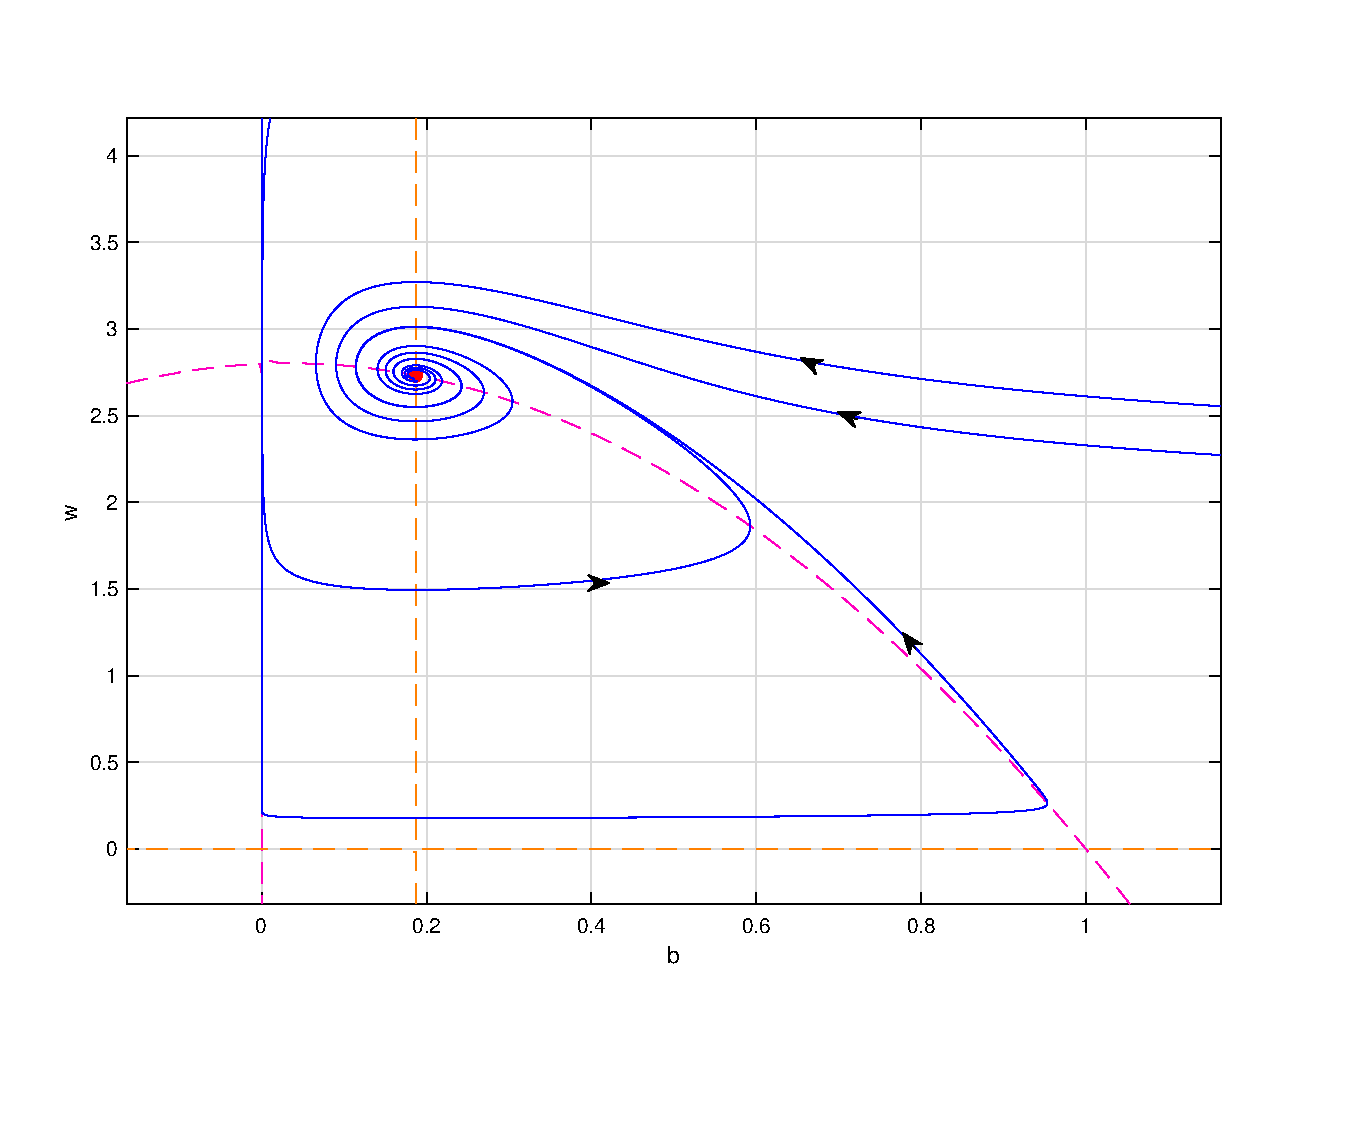
\includegraphics[scale=0.3]{FIGURES/s.eps}  

\end{center}

\caption{Figure shows sample runs of $b(t)$ and $w(t)$ for equations
  (\ref{eq:scaledODE1}) and (\ref{eq:scaledODE2}), where
  $p(\theta )$ = 3, where the system is stable }
      \label{fig:S}
\end{figure}
%%%%%%%%%%%%%%%%%%%%%%%%%%%%%%%%%%%%%%%%%%%%
\begin{figure}[!htp]
\begin{center}
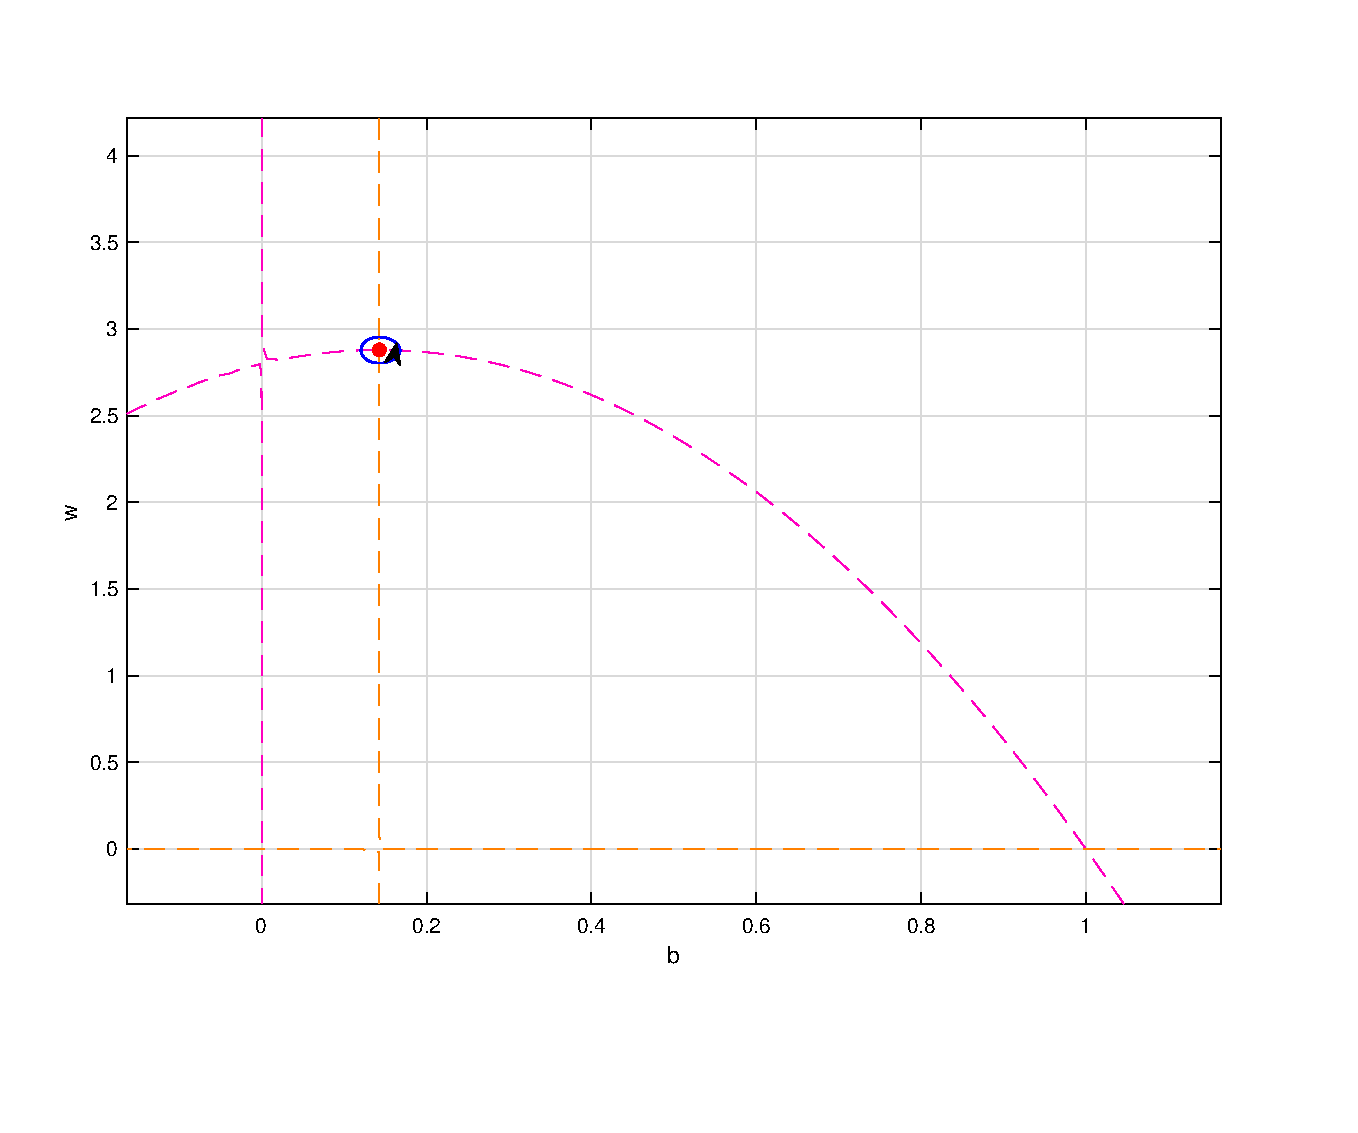
\includegraphics[scale=0.28]{FIGURES/l1.eps}  
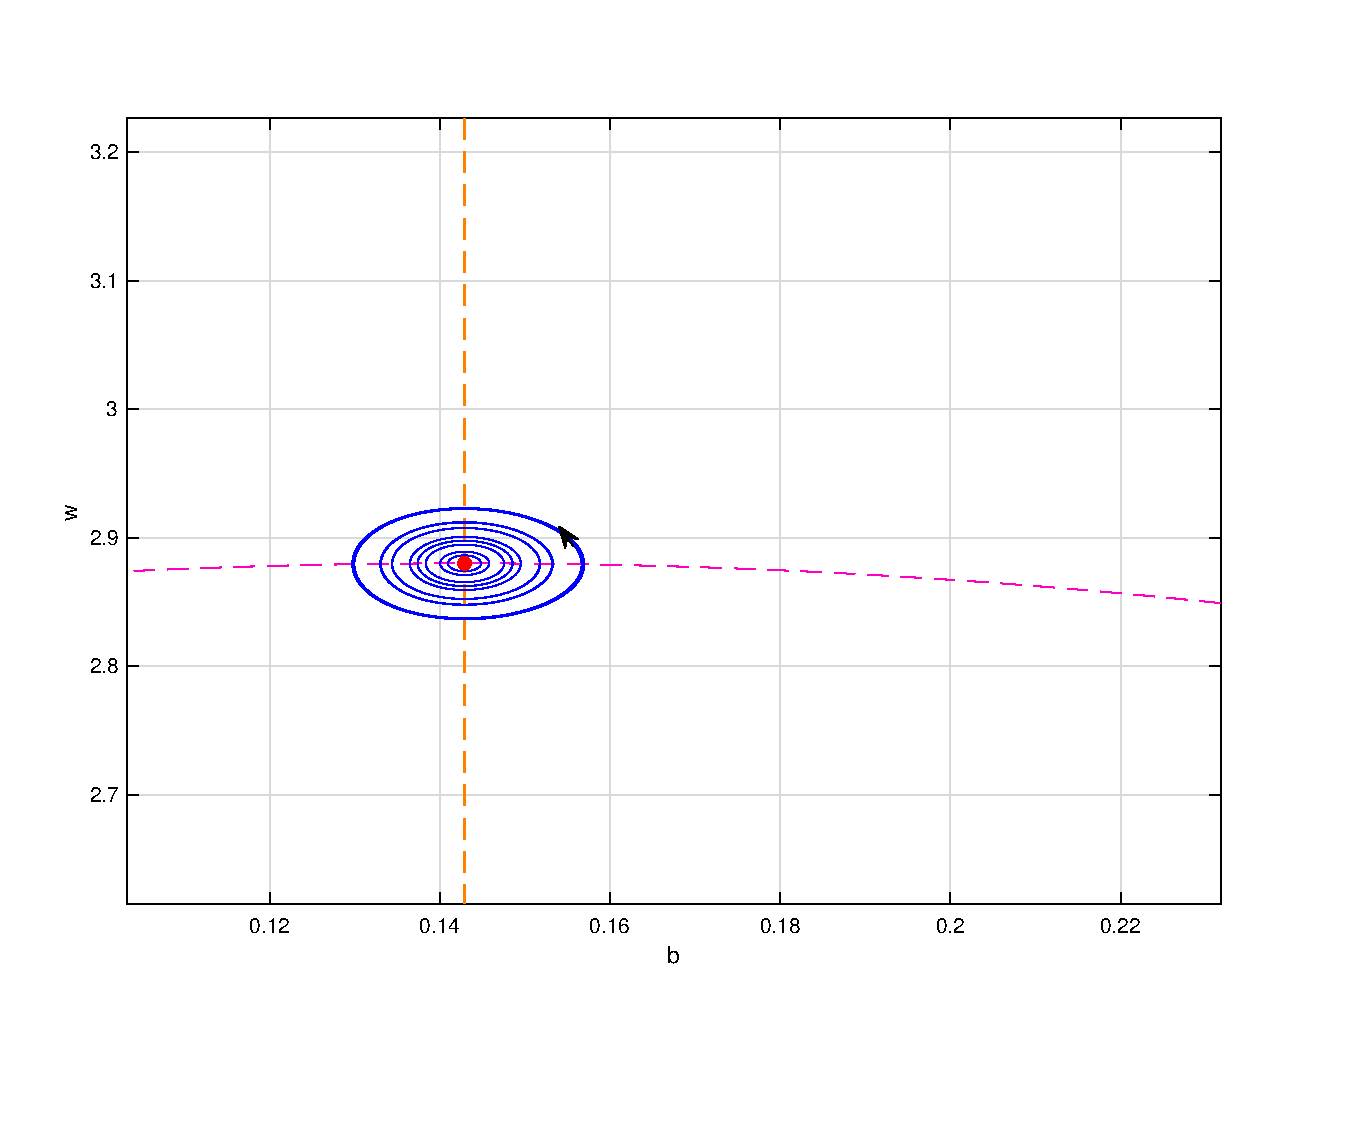
\includegraphics[scale=0.28]{FIGURES/l2.eps}

\end{center}

\caption{Figure shows runs of $b(t)$ and $w(t)$ for equations
  (\ref{eq:scaledODE1}) and (\ref{eq:scaledODE2}) has center
  equilibrium point, where $p(\theta )=3.92$. }
      \label{fig:l1l2}
\end{figure}

In the next theorem we aim to investigate the effect of the impact
associated with the use of the anti-pheromone $p(\theta )$ on
the limit cycle dynamics in equations (\ref{eq:scaledODE1}) and
(\ref{eq:scaledODE2}).

\begin{theorem}
  \index{4} Consider the model equations (\ref{eq:scaledODE1}) and
  (\ref{eq:scaledODE2}). Assume that $E^{\ast }=(b^{\ast },w^{\ast })$
  is the positive non trivial equilibrium point of the model equations
  (\ref{eq:scaledODE1}) and (\ref{eq:scaledODE2}) with \ $g>d$ and the
  following condition hold
\end{theorem}

\begin{center}
$%
p(\theta )>c+\dfrac{2cd}{g-d}>0,$
\end{center}

then the system possesses at least one closed loop in the first quadrant.

\begin{proof}
  From the local stability analysis, we have that if the above
  conditions hold, then the positive equilibrium
  $E^{\ast }=(b^{\ast },w^{\ast })$ of equations (\ref{eq:scaledODE1})
  and (\ref{eq:scaledODE2}) is an unstable node or focus. The
  existence of a closed loop now follows from Lemma \ref{mm} and
  Poincair{\`e}--Bendixson theorem \citep{nonlinearChaos}.
\end{proof}

\begin{figure}[!htp]
\begin{center}
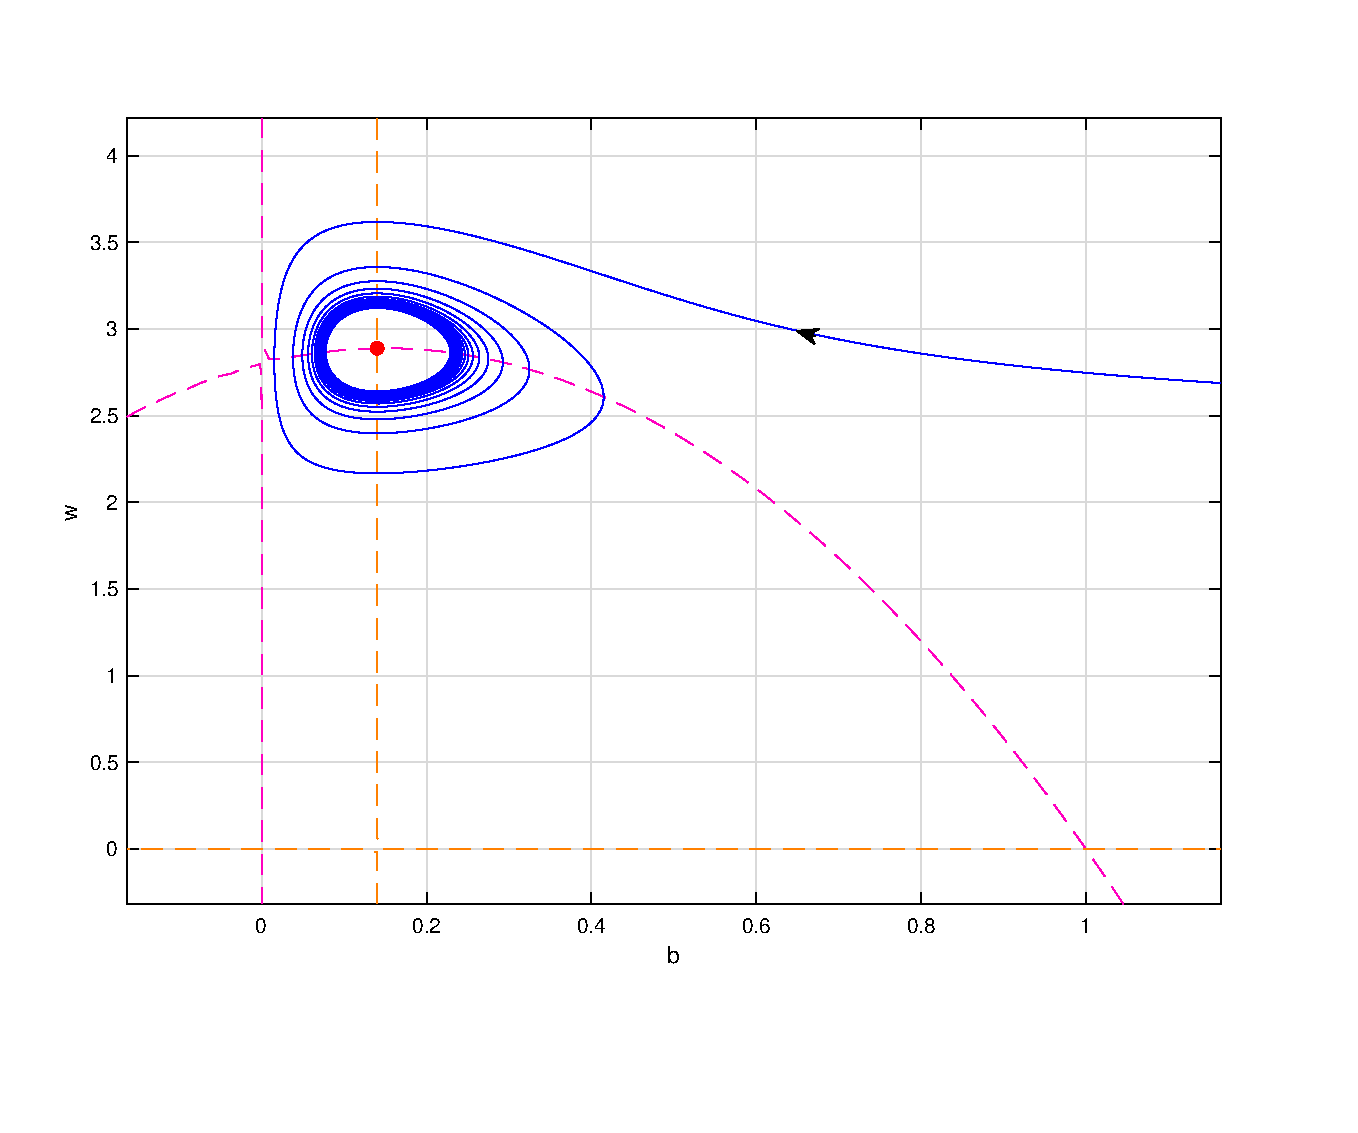
\includegraphics[scale=0.3]{FIGURES/lim.eps}  

\end{center}

\caption{Figure shows sample runs of $b(t)$ and $w(t)$ for equations
  (\ref{eq:scaledODE1}) and (\ref{eq:scaledODE2}) , where
  $p(\theta )$ = 4, where the system has a limit cycle }
      \label{fig:lim}
\end{figure}

\fi

\section{Numerical Approximations}
\label{numericalApproximationODE}
\subsection{Numerical Approximations of the ODE system}
The system of ODEs given in
equations (\ref{eq:scaledODE1}) and (\ref{eq:scaledODE2}) was
approximated using a Runga-Kutta Fehlberg method with a minimum step
size of 1.0E-5. 
The approximation for the initial value of $m$ was started near the
non-trivial steady state, but the values of the butterflies and wasps
were taken to be 95\% of the values for the steady state. The
approximation was run until it detected the state was not changing or
a limit cycle was reached. In this case, if both densities did not
change more than 1.0E-7 from a previous high or low value for over
2000 time steps it was considered to be at a steady state. For the
limit cycle if the minimum and maximum for both densities was within
1.0E-7 for two full cycles then it was considered to be in a limit
cycle.

After the initial approximation, the initial condition for the next
value of $m$ was the end state of the previous approximation. This
process was done for the values of $m$ starting at the lowest value
and increasing. the process was then repeated for the value of $m$
starting at the highest value and decreasing. The results were nearly
identical, and no hysteresis was detected.
\subsection{Numerical Approximations of the Coupled PDE and ODE system}
\label{numericalApproximation}

We introduce the method for the numerical approximation of the coupled
PDE and ODE system in equations (\ref{eq:scaledodePDE1}) and
(\ref{eq:scaledodePDE2}). For the full system, we make use of a
Legendre pseudo-spectral collocation
method\citep{spectralMethodsFluids,hesthaven_gottlieb_gottlieb_2007,gottlieb1977numerical}. First,
the butterfly density is discretized in $\theta$ as
\begin{eqnarray}
  \label{eqn:spatialDiscretization}
  b_N(t,\theta) & = & \sum^N_{i=0} \hat{b}_i(t) \phi_i(\theta),
\end{eqnarray}
where $\phi_i(\theta)$ is the Lagrange interpolant on the
$i$\textsuperscript{th} abscissa of the Legendre-Gauss-Lobatto
quadrature\citep{hesthaven_gottlieb_gottlieb_2007}.

The abscissa of the Legendre-Gauss-Lobatto quadrature are the zeroes
of the function
\begin{eqnarray}
  \psi(\theta) & = & \left(1-\theta^2\right) L_{N}'(\theta),
\end{eqnarray}
where $L_N(\theta)$ is the $n$\textsuperscript{th} Legendre
polynomial\citep{davis2007methods}.  The weights, $w_n$, associated
with the quadrature are identical to those described in
Davis\citep{davis2007methods} as well as Golub and
Welsch\citep{gaussQuadratureRules}. In our examples the quadrature is
approximated using the methods described by Golub and
Welsch\citep{gaussQuadratureRules}.  Given $\psi(\theta)$ the Lagrange
interpolants can be calculated
\begin{eqnarray}
  \phi_i(\theta) & = & \frac{\psi(\theta)}{\psi'(\theta)(\theta-\theta_i)}.
\end{eqnarray}
The function $\psi(\theta)$ coincides with the Legendre differential
equation, and the relationship can be simplified as
\begin{eqnarray}
  \psi'(\theta) & = & -N(N+1)L_N(\theta).
\end{eqnarray}

The discretization of equations (\ref{eq:scaledodePDE1}) and
(\ref{eq:scaledodePDE2}) is constructed by substituting the definitionhttps://www.overleaf.com/project/5eb9da10e929ab0001816b1e
of $b_N$ from equation (\ref{eqn:spatialDiscretization})https://www.overleaf.com/project/5eb9da10e929ab0001816b1e. A Galerkin
approximation is constructed, and one minor complication is that the
Lagrange interpolants are polynomials of degree $N$, and the
Gauss-Lobatto quadrature is exact for polynomials up to degree
$N$. The integral is approximated using the Gauss-Lobatto quadrature,
and the resulting sum results in an equivalent norm compared to the
Gauss quadrature which is exact for polynomials up to degree
$N$\citep{SobolevCanutoQuarteroni}.

The resulting variational form for Neumann boundary conditions using a
Galerkin approximation and a discrete inner product for equation
(\ref{eq:scaledodePDE1}) is
\begin{eqnarray}
  \sum_{j=0}^N \sum_{i=0}^N  \hat{b}_i'(t) \phi_i(\theta_j) \phi_k(\theta_j) w_j
  & = &
  \sum_{j=0}^N \sum_{i=0}^N p(\theta_j)  \hat{b}_i(t) (1 - \hat{b}_i(t) ) \phi_i(\theta_j) \phi_k(\theta_j) w_j \\
  & &  -  \sum_{j=0}^N w(t) \frac{p(\theta_j) \sum_{i=0}^N \hat{b}_i(t) \phi_i(\theta_j) }{c+p(\theta_j) \sum_{i=0}^N \hat{b}_i(t) \phi_i(\theta_j)} \phi_k(\theta_j) w_j \nonumber \\ 
  & & - \sum_{j=0}^N \mu  \sum_{i=0}^N \hat{b}_i(t) \phi_i'(\theta_j) \phi_k'(\theta_j)  w_j, \nonumber
\end{eqnarray}
for all integer values of $k$ from $0$ to $N$ inclusive.  The basis
functions are the Lagrange interpolants on the abscissa, and the
equations can be reduced to
\begin{eqnarray}
  \hat{b}_k'(t) 
  & = &
        p(\theta_j) \hat{b}_k(t) (1 - \hat{b}_k(t) )
        -  w(t) \frac{p(\theta_k) \hat{b}_k(t)) }{c+p(\theta_k)  \hat{b}_k(t) }  
   - \frac{\mu}{w_k} \sum_{i=0}^N \hat{b}_i(t) \left( \sum_{j=0}^N  \phi_i'(\theta_j) \phi_k'(\theta_j)  w_j \right).
\end{eqnarray}
The corresponding discretization of the equation for the wasps is can be simplified because the moth population is defined on the Gauss-Labotto points,and the integral can be approximated as described above. A similar approach has been described by \cite{doi:10.1002/mma.1318}.

Combined with equation (\ref{eq:scaledodePDE2}) the approximation
consists of a system of $N+2$ ordinary differential equations. The
integral in equation (\ref{eq:scaledodePDE2}) is approximated using
the Legendre-Gauss-Lobatto quadrature. The temporal discretization of
the resulting system is constructed using a second order, implicit
multi-step scheme. The scheme is implemented as a fully implicit
second order Adams-Moulton scheme\citep{ascher2011first}. At each time
step the resulting non-linear system is approximated using Newton's
method.



\clearpage
%\bibliographystyle{siam}
\bibliographystyle{elsarticle-harv}
\bibliography{animalBehaviour}



\end{document}

https://www.overleaf.com/project/5eb9da10e929ab0001816b1e
